\documentclass[11pt,a4paper]{article}
\usepackage[T1]{fontenc}
\usepackage{lmodern}
\usepackage{graphicx}
\usepackage{amsmath,amssymb}
\usepackage{hyperref}
\usepackage{listings}
\usepackage{geometry}
\usepackage{booktabs}
\usepackage{longtable}
\usepackage{xcolor}
\usepackage{float}
\geometry{margin=2.3cm}
\hypersetup{colorlinks=true,linkcolor=blue,urlcolor=blue,citecolor=blue}
\lstset{basicstyle=\ttfamily\small,breaklines=true,frame=single,columns=fullflexible}

\title{BioTraj\\User Manual\\Version 1.2}
\author{Danilo Roccatano\\School of Engineering and Physical Sciences\\University of Lincoln}
\date{September 2026}

\begin{document}
\maketitle
\tableofcontents
\newpage

\section{Introduction}
BioTraj (BioTrajectoryAnalysis) is an open-source collection of Python tools for extracting and quantitatively analysing biological trajectories from video recordings. The framework combines computer vision, automated tracking, conventional trajectory descriptors, and information-geometric analysis of spatially and temporally resolved movement distributions.

The software was initially developed for ant trajectory analysis, but the workflow can be adapted to other organisms and moving agents provided that suitable two-dimensional trajectories can be obtained. Tracking and analysis are separated through CSV trajectory files, so trajectories generated by other tracking programs can also be analysed.

The current release contains two principal components:
\begin{enumerate}
\item \texttt{AntTracking.py}: video-based trajectory extraction;
\item \texttt{AntTrajectoryAnalysis.py}: conventional trajectory analysis together with spatial and temporal Fisher--Rao information geometry.
\end{enumerate}
Companion utilities provide scene annotation and annotation-aware analysis, while a synthetic trajectory generator provides controlled validation datasets. These utilities are described later in this manual.

\section{Software Architecture}
The BioTraj workflow is modular (Figure~\ref{fig:architecture}). Video acquisition and computer-vision tracking are separated from quantitative trajectory analysis through an intermediate CSV trajectory file. The tracking stage is implemented by \texttt{AntTracking.py}, whereas the principal analysis stage is implemented by \texttt{AntTrajectoryAnalysis.py}. This separation allows BioTraj to analyse trajectories produced by other tracking programs, provided that they are converted to the expected CSV representation, and permits new analysis methods to be added without modifying the tracking module.

The analysis engine provides conventional spatial and dynamical descriptors and, when requested, spatial and temporal information-geometric analyses. Scene annotation and annotation-aware Fisher--Rao analysis are implemented as companion modules described later in this manual.

\begin{figure}[H]
\centering
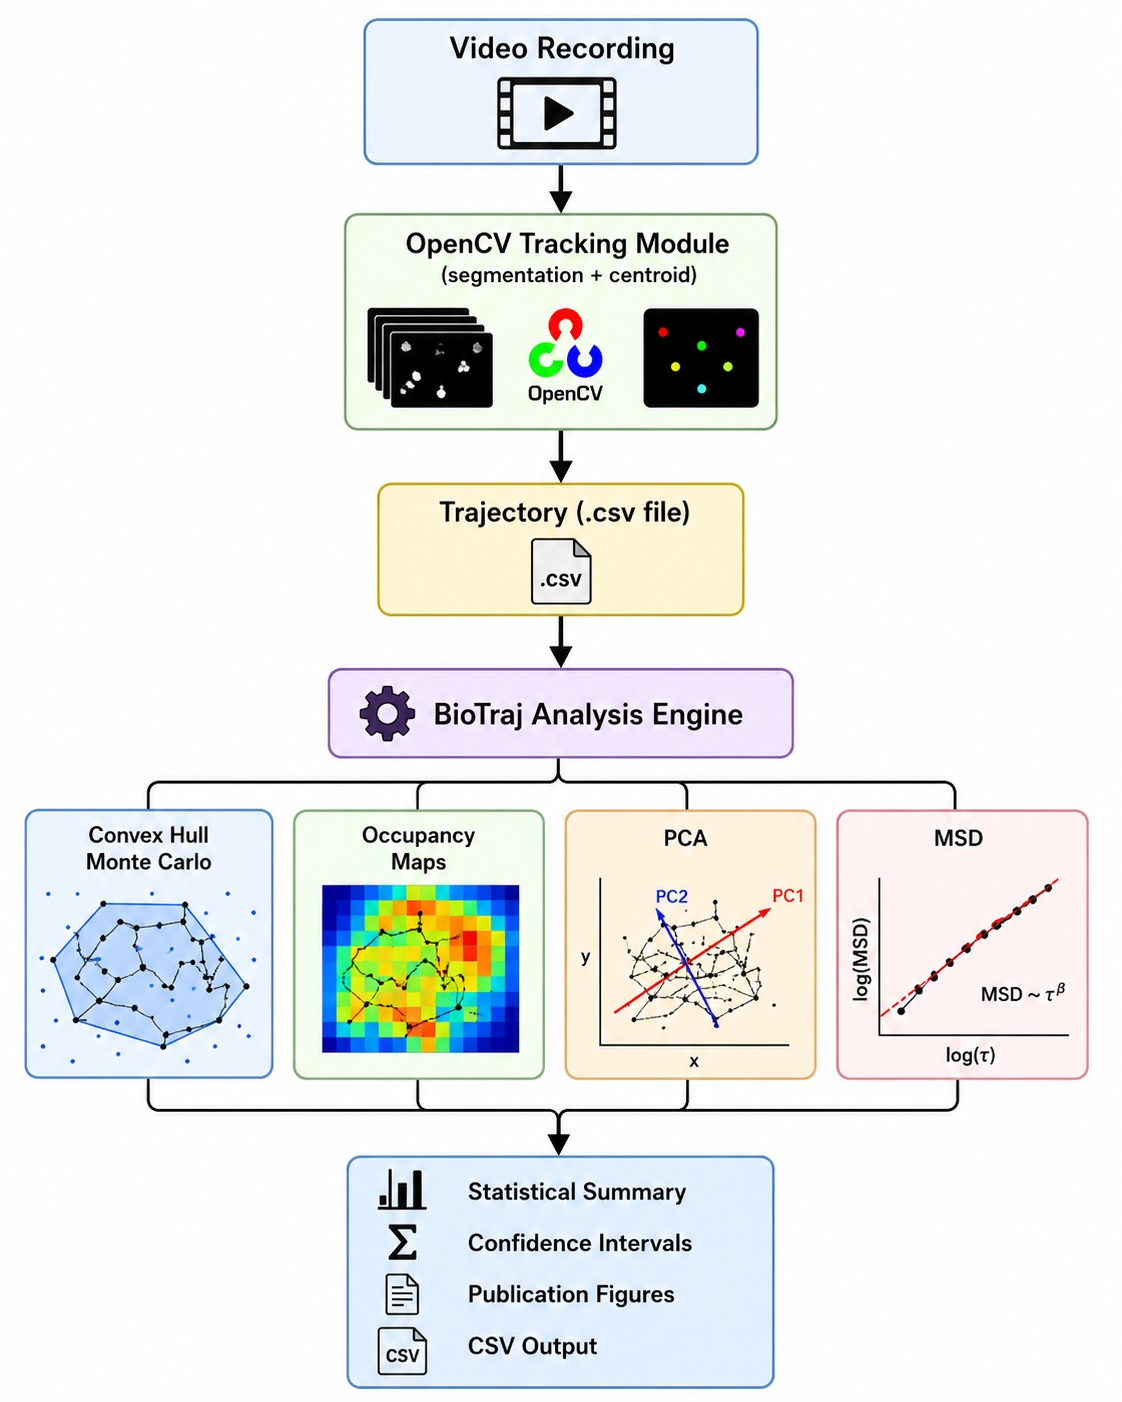
\includegraphics[width=0.78\textwidth]{figures/architecture.jpg}
\caption{\textbf{BioTraj software architecture.} A video recording is processed by the computer-vision tracking module (\texttt{AntTracking.py}) to produce trajectory coordinates in CSV format. The trajectory file is then analysed by the BioTraj analysis engine (\texttt{AntTrajectoryAnalysis.py}). The diagram illustrates representative conventional outputs, including explored-area estimates, occupancy maps, PCA-based anisotropy and mean-squared-displacement analysis. Spatial and temporal Fisher--Rao information geometry and the companion annotation-aware analysis extend this core workflow and are described in later sections.}
\label{fig:architecture}
\end{figure}

\section{Installation}
BioTraj requires Python 3.10 or newer. Principal dependencies include OpenCV, NumPy, Pandas, SciPy, Matplotlib, and scikit-learn. Install repository requirements using:
\begin{lstlisting}
pip install -r requirements.txt
\end{lstlisting}

\section{Coordinate System}
Video images follow the OpenCV convention, with the origin at the upper-left corner. Statistical analyses and graphical outputs may transform coordinates to a Cartesian representation with the origin at the lower-left, the $x$ axis increasing to the right, and the $y$ axis increasing upwards. Users should retain the original image coordinate system when defining scene annotations intended to overlay the video frame.

\section{Trajectory Extraction}
\subsection{Overview}
The tracking program detects moving objects, filters detections, associates detections between frames, reconstructs continuous track segments, and writes coordinates to a CSV file. A tracking identifier denotes a continuous reconstructed track segment; it should not automatically be interpreted as a persistent biological individual when identities can be lost or exchanged.

\subsection{Basic Usage}
\begin{lstlisting}
python3 AntTracking.py video.mov
\end{lstlisting}
A typical configured run is:
\begin{lstlisting}
python3 AntTracking.py video.mov \
    --threshold 18 \
    --min-area 6 \
    --max-area 250 \
    --output tracking_results
\end{lstlisting}
Important tracking parameters include the detection threshold, minimum and maximum object area, maximum association distance, maximum permitted track gap, and merge distance. Appropriate values depend on image scale, contrast, frame rate, and organism size.

\section{Trajectory Data Format}
The analysis program accepts trajectory data in CSV format. A typical file contains:
\begin{lstlisting}
track_id,frame,x,y
1,0,123.4,201.7
1,1,124.2,202.3
1,2,125.0,203.1
\end{lstlisting}
Coordinates may be expressed in pixels or calibrated physical units. Turning angles are calculated only within uninterrupted track segments and are never bridged across missing portions of a trajectory.

\section{Trajectory Analysis}
\subsection{Basic Usage}
The current analysis program is run with the trajectory CSV as the positional argument:
\begin{lstlisting}
python3 AntTrajectoryAnalysis.py \
    ant_tracks.csv \
    --output analysis_results
\end{lstlisting}
Without information-geometry switches, the program provides the conventional BioTraj trajectory descriptors and associated figures.

\subsection{Conventional Descriptors}
BioTraj calculates complementary geometric and dynamical descriptors, including convex-hull explored area, Monte Carlo area estimation, occupancy maps, principal-component anisotropy, mean-squared displacement (MSD), straightness, and fractal dimension. Figure~\ref{fig:conventional-workflow} illustrates how these descriptors fit into the experimental workflow, from video recording and object tracking to reconstructed trajectories and quantitative analysis.

\begin{figure}[H]
\centering
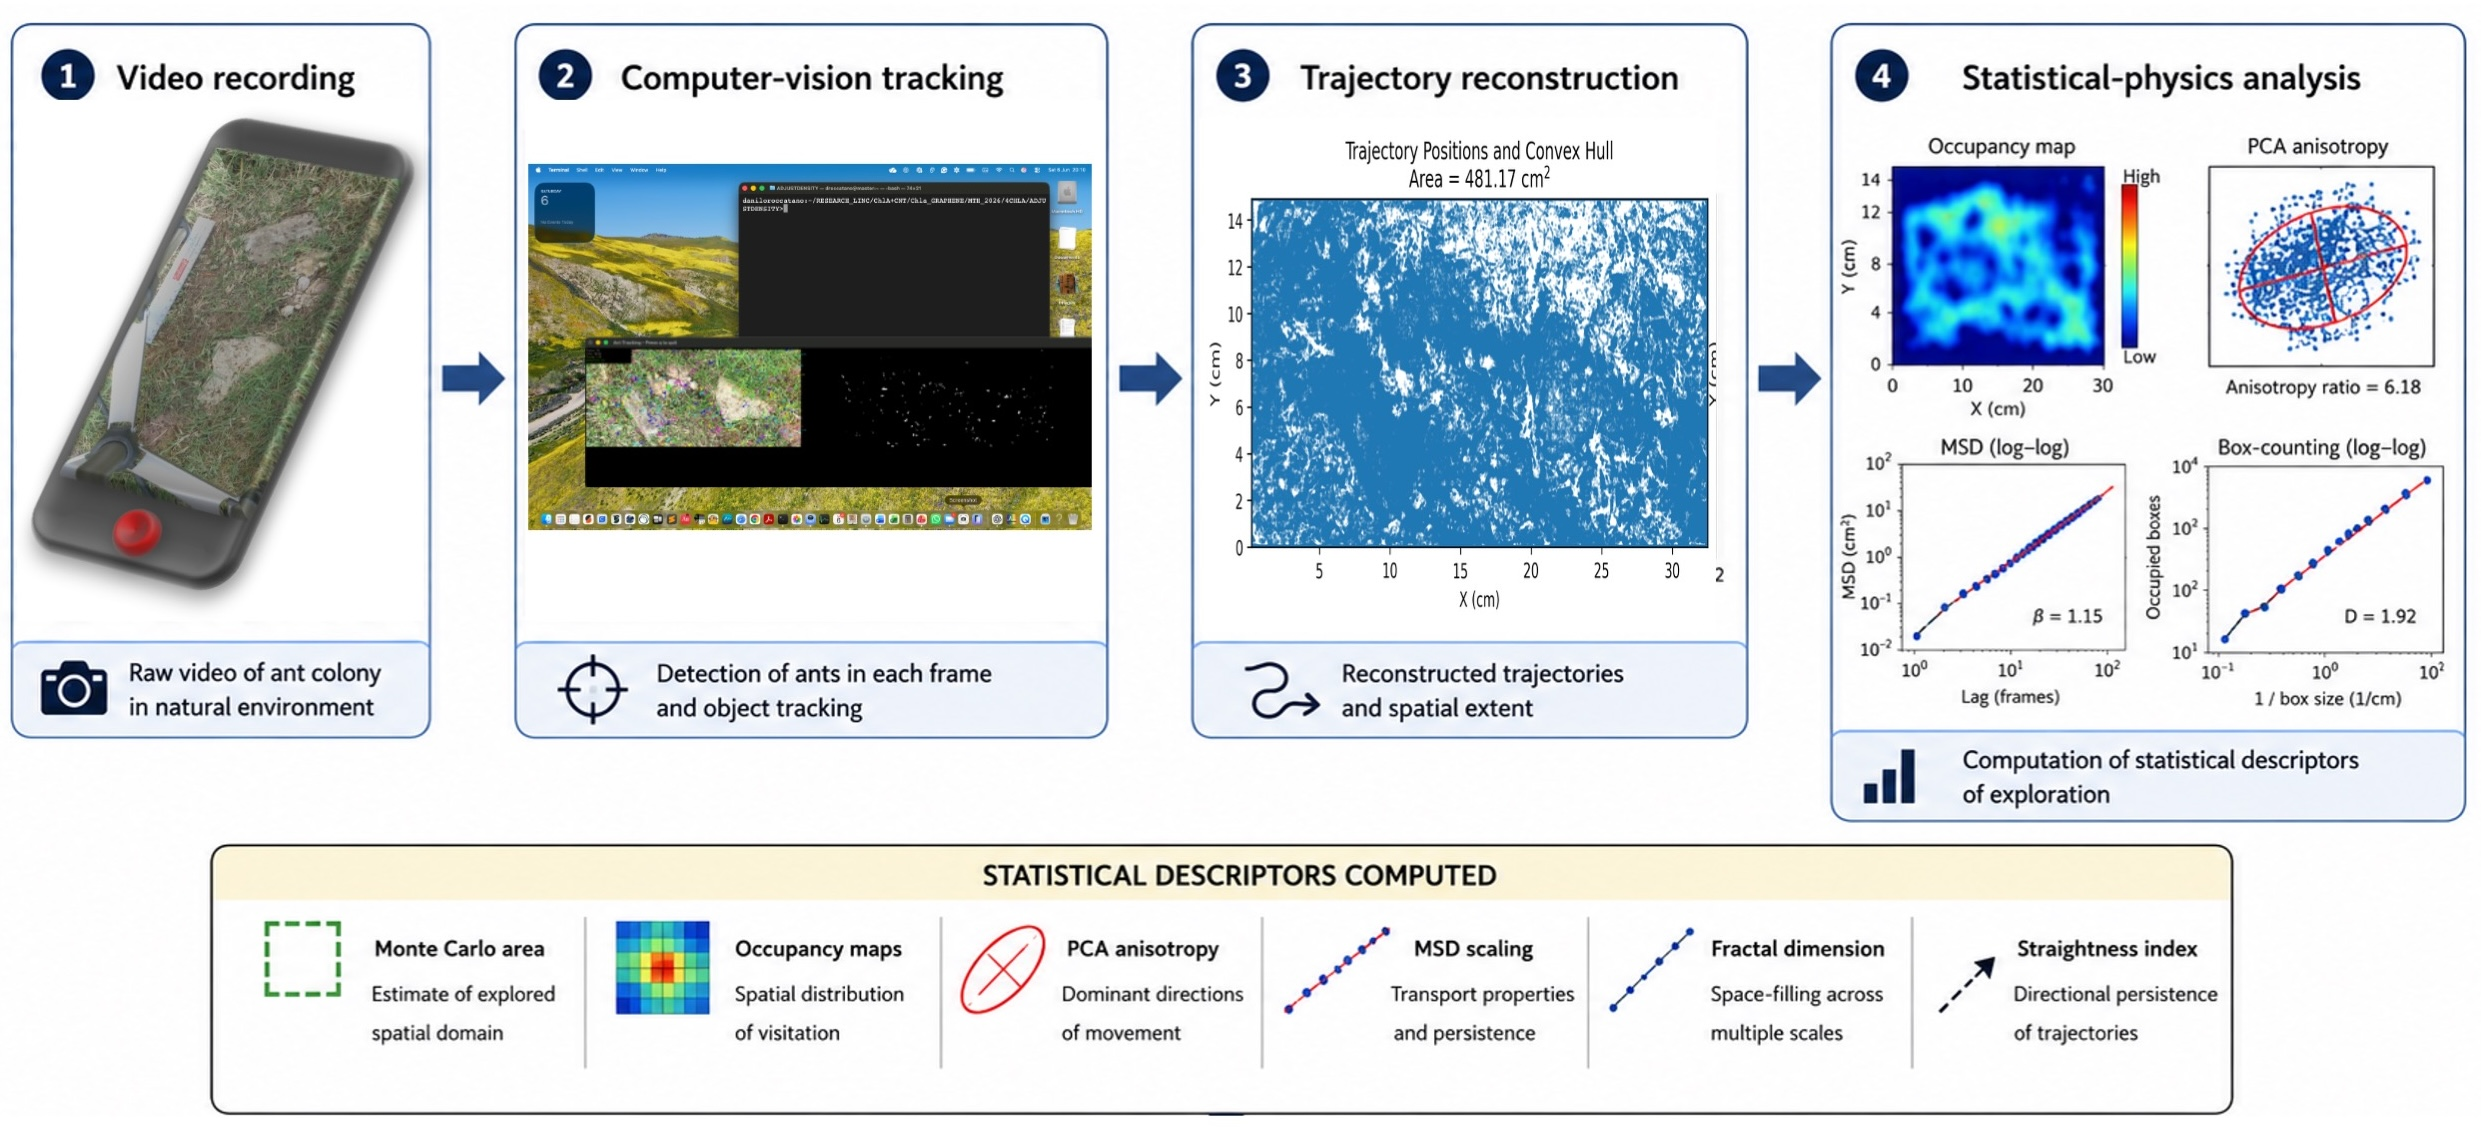
\includegraphics[width=\textwidth]{figures/conventional_analysis_workflow.jpg}
\caption{\textbf{From video recording to conventional BioTraj descriptors.} A biological recording is processed by computer-vision tracking to reconstruct trajectories and their spatial extent. BioTraj then calculates complementary descriptors of spatial exploration and movement dynamics. Representative outputs shown here include occupancy maps, PCA anisotropy, MSD scaling, box-counting fractal dimension, Monte Carlo area estimation and trajectory straightness. The figure illustrates the conventional-analysis branch of BioTraj; the information-geometric analyses described later provide additional spatially and temporally resolved comparisons of movement distributions.}
\label{fig:conventional-workflow}
\end{figure}

\subsubsection{Explored Area and Monte Carlo Estimation}
The explored domain is approximated by the convex hull. A Monte Carlo estimate can be obtained from random points within a bounding rectangle:
\begin{equation}
A_{\mathrm{MC}}=A_{\mathrm{box}}\frac{N_{\mathrm{inside}}}{N_{\mathrm{total}}}.
\end{equation}

\subsubsection{Principal Component Analysis}
For trajectory positions $\mathbf r_i$, the covariance matrix is diagonalized to obtain eigenvalues $\lambda_1$ and $\lambda_2$. The anisotropy ratio is
\begin{equation}
A=\frac{\lambda_1}{\lambda_2}.
\end{equation}
Values near unity indicate approximately isotropic spatial exploration; larger values indicate an increasingly elongated spatial distribution.

\subsubsection{Mean-Squared Displacement}
\begin{equation}
\mathrm{MSD}(\tau)=\left\langle |\mathbf r(t+\tau)-\mathbf r(t)|^2\right\rangle.
\end{equation}
When an approximate power law $\mathrm{MSD}(\tau)\propto\tau^\beta$ is observed, $\beta<1$ corresponds to sublinear/subdiffusive scaling, $\beta\approx1$ to diffusive scaling, and $\beta>1$ to superlinear/superdiffusive scaling. Superlinear scaling can arise from persistent or otherwise correlated motion and should not be assigned a unique mechanism from $\beta$ alone.

\subsubsection{Straightness and Fractal Dimension}
Straightness compares net displacement with total path length. Fractal dimension provides a complementary measure of trajectory complexity and space-filling character over the analysed scales.

\begin{figure}[H]
\centering
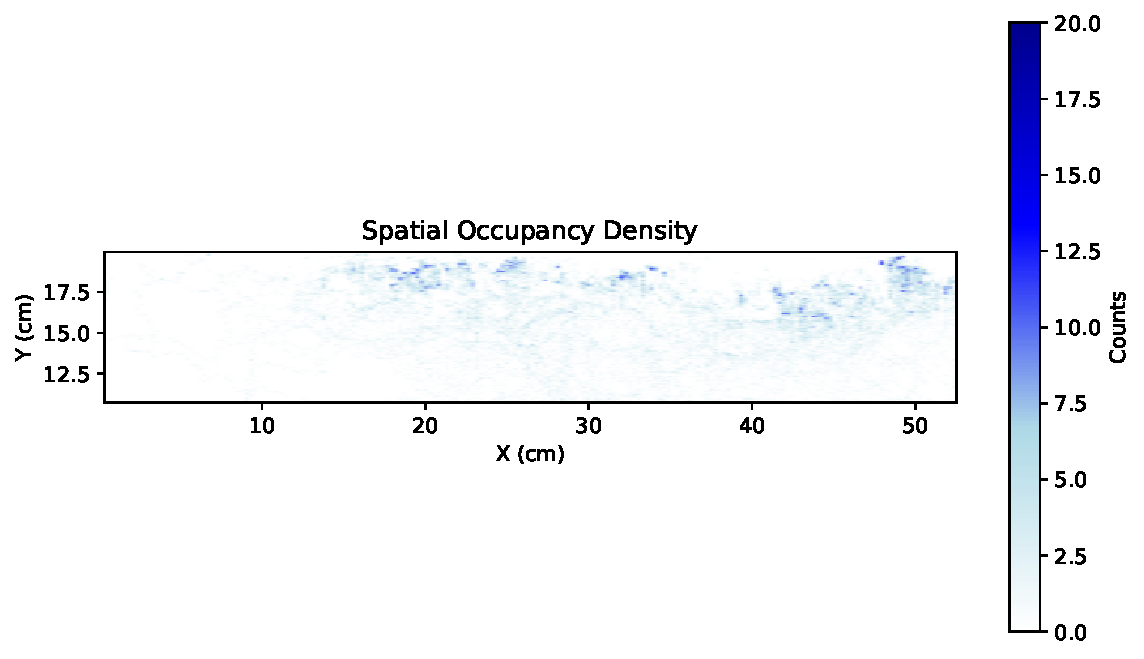
\includegraphics[width=0.82\textwidth]{figures/density_heatmap.pdf}
\caption{Example BioTraj occupancy map. Occupancy describes \emph{where} observations occur and is complementary to the information-geometric analysis, which describes how local movement distributions differ.}
\label{fig:occupancy}
\end{figure}

\section{Information-Geometric Analysis}
\subsection{Purpose and Interpretation}
The information-geometric module detects spatial or temporal changes in empirical movement distributions without requiring predefined behavioural states. The present implementation uses unsigned turning-angle distributions.

\textbf{Important interpretation rule:} Fisher--Rao heterogeneity identifies where or when estimated movement statistics change; it does not determine why they change. Elevated values may reflect biological responses, physical constraints, surface geometry, projection effects, tracking artefacts, finite sampling, or combinations of these factors.

\subsection{Turning-Angle Distributions}
For three consecutive positions in the same continuous track segment,
\begin{equation}
\Delta\mathbf r_t=\mathbf r_{t+1}-\mathbf r_t,
\end{equation}
and the unsigned turning angle is
\begin{equation}
\Delta\theta_t=\arccos\left(
\frac{\Delta\mathbf r_{t-1}\cdot\Delta\mathbf r_t}
{\|\Delta\mathbf r_{t-1}\|\,\|\Delta\mathbf r_t\|}
\right),\qquad 0\leq\Delta\theta\leq\pi.
\end{equation}
Within a spatial cell or temporal window, the angles are converted to a normalized histogram on a fixed common angular partition,
\begin{equation}
P=(p_1,\ldots,p_K),\qquad p_k\geq0,\qquad \sum_{k=1}^{K}p_k=1.
\end{equation}

\subsection{Fisher--Rao Distance}
The square-root embedding
\begin{equation}
\psi(P)=2\left(\sqrt{p_1},\ldots,\sqrt{p_K}\right)
\end{equation}
maps the categorical probability simplex isometrically, under the Fisher
metric convention used by BioTraj, to the positive orthant of a sphere of
radius 2 because $\|\psi(P)\|_2=2$. Equivalently, the unscaled square-root
vector $(\sqrt{p_1},\ldots,\sqrt{p_K})$ lies on the unit sphere. Under this
convention, the Fisher--Rao geodesic distance between two categorical
distributions is
\begin{equation}
d_{\mathrm{FR}}(P,Q)=
2\arccos\left(\sum_{k=1}^{K}\sqrt{p_kq_k}\right).
\end{equation}
Thus $0\leq d_{\mathrm{FR}}\leq\pi$, with zero corresponding to identical
distributions and $\pi$ to distributions with disjoint support. The same
fixed histogram partition must be used when distributions are compared.

\subsection{Spatial Information Geometry}
With \texttt{--info-geometry}, the analysed domain is divided into a rectangular grid. A turning-angle distribution is estimated for each sufficiently sampled cell. Pairwise Fisher--Rao distances quantify statistical separation between cells, while the local Fisher--Rao heterogeneity assigned to a cell summarizes its distances from valid neighbouring cells.

Large local values indicate that a cell's estimated turning-angle distribution differs strongly from those of its neighbours. Small values indicate locally similar distributions.

\begin{figure}[H]
\centering
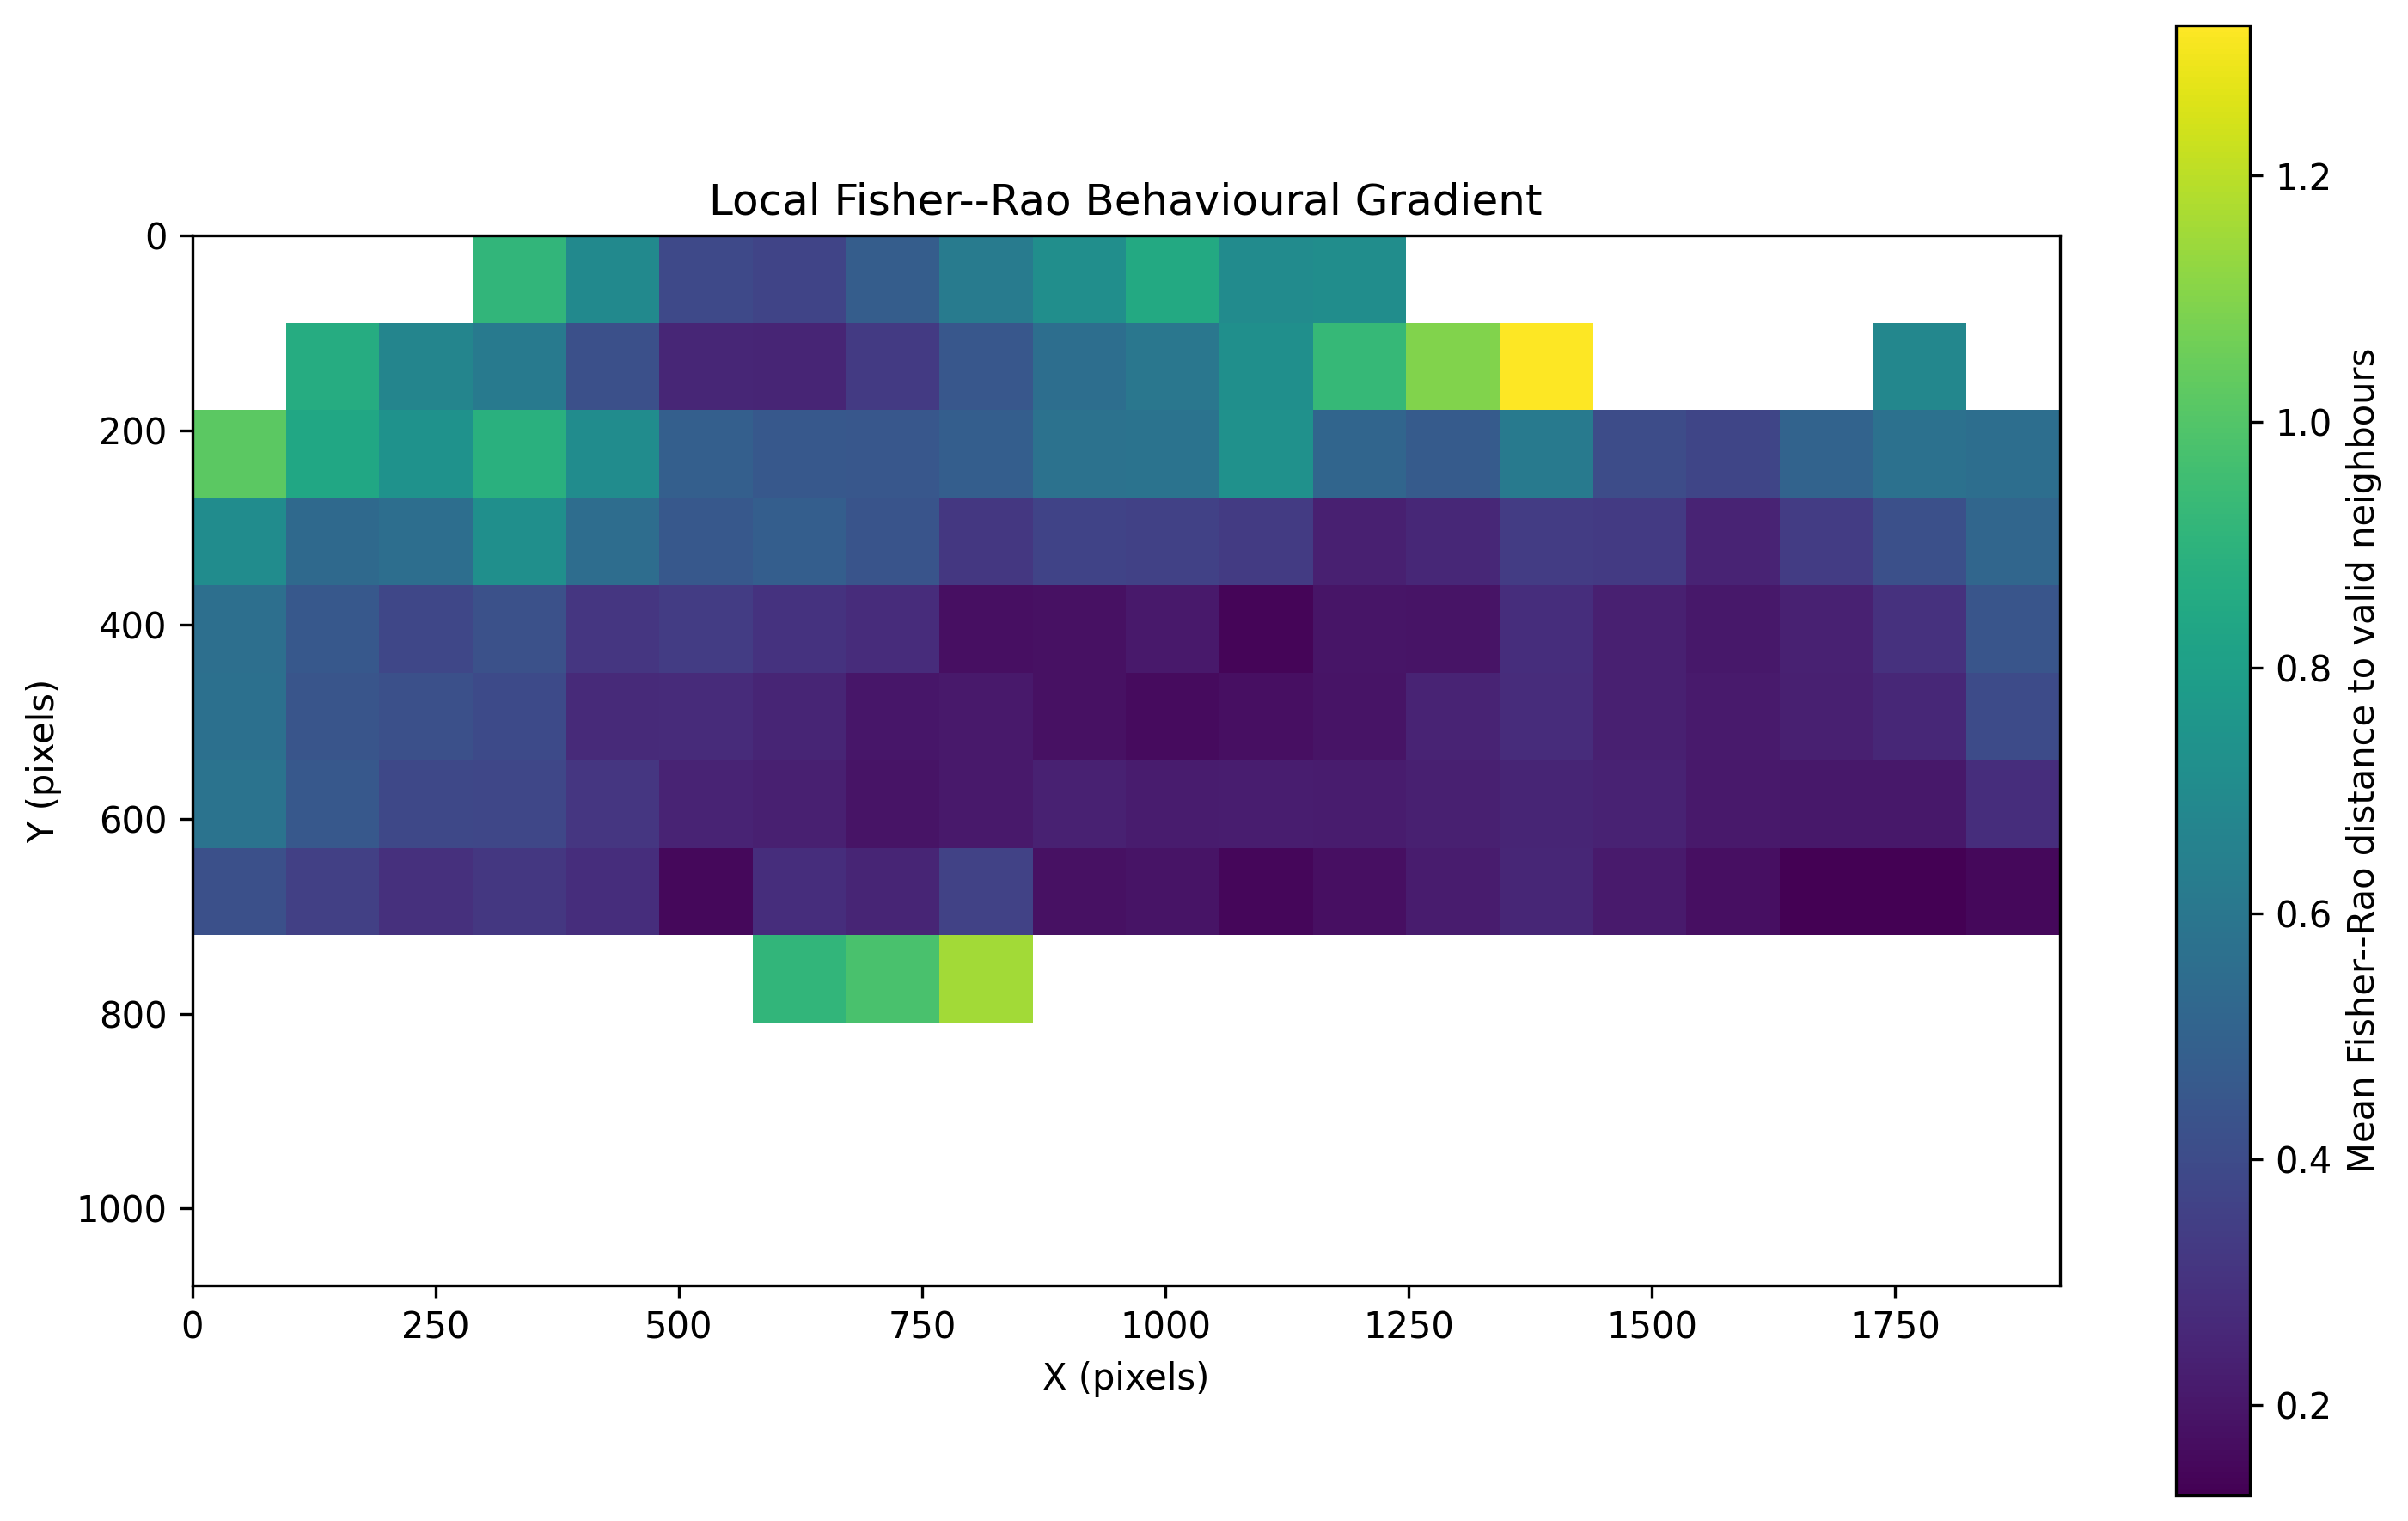
\includegraphics[width=0.78\textwidth]{figures/info_geometry_local_gradient.png}
\caption{Example spatial Fisher--Rao map. Colour represents local Fisher--Rao heterogeneity calculated from neighbouring spatial cells. The map identifies spatial changes in movement statistics and should not be interpreted automatically as a behavioural-state map.}
\label{fig:localfr}
\end{figure}

\begin{figure}[H]
\centering
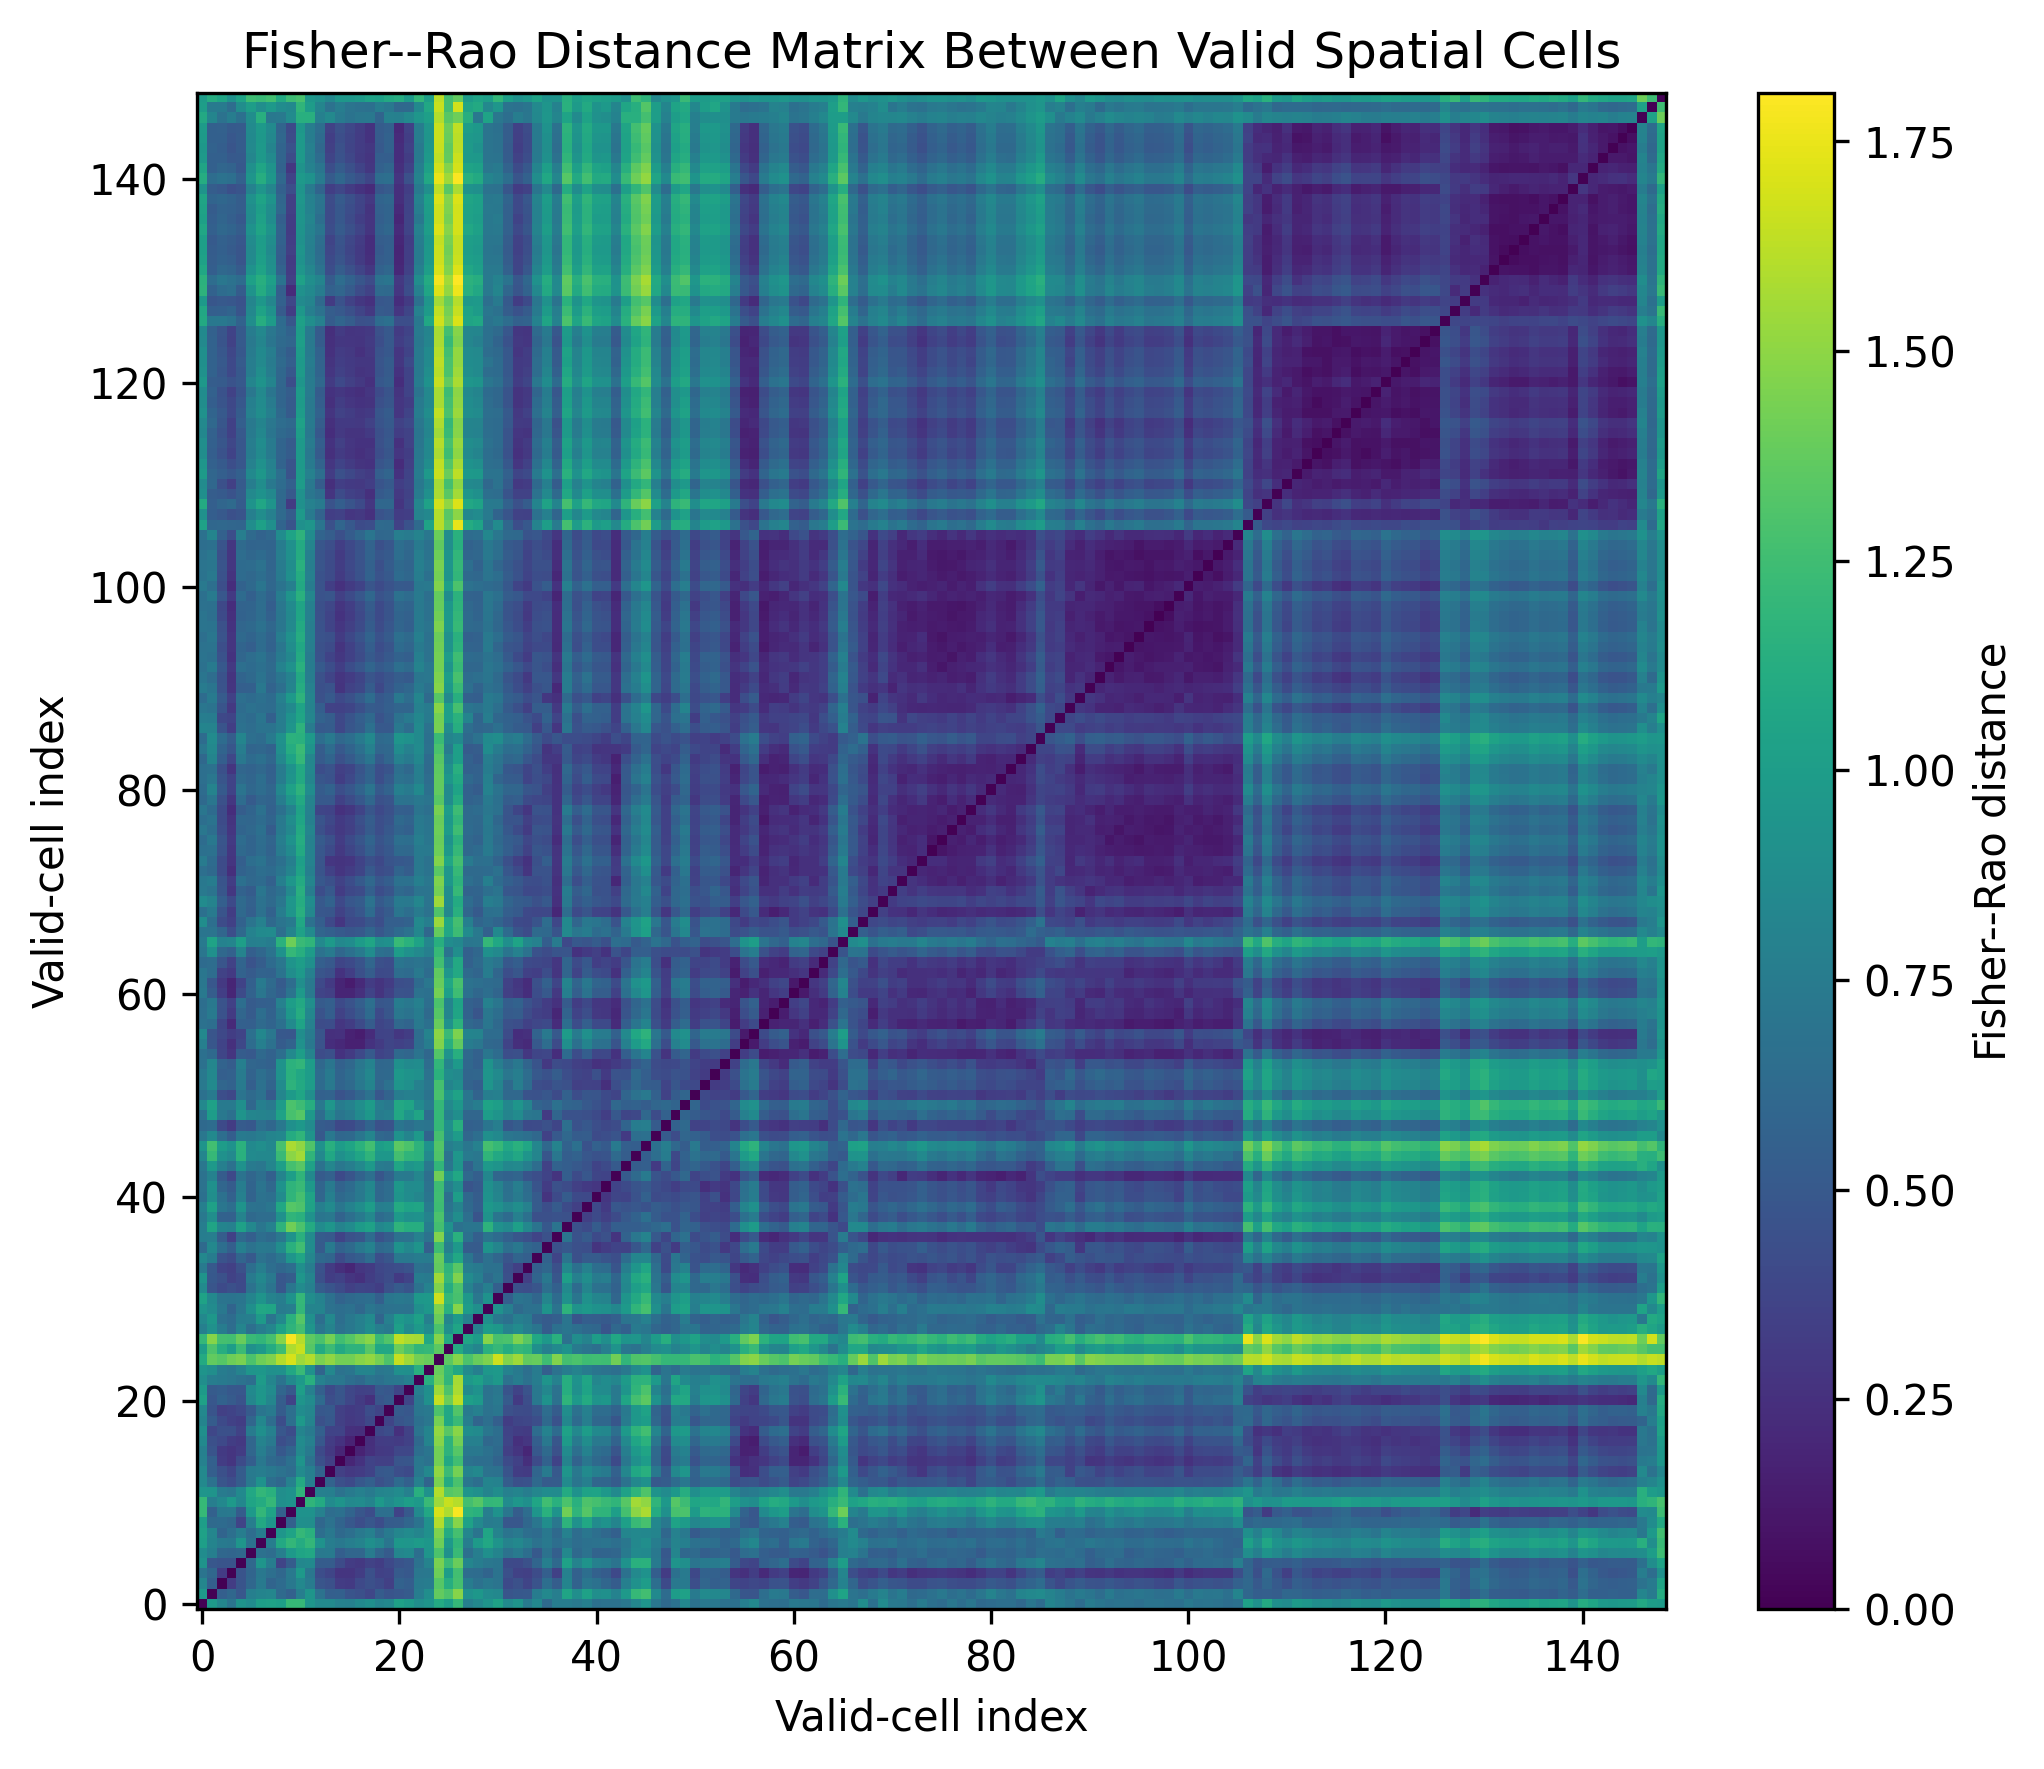
\includegraphics[width=0.72\textwidth]{figures/info_geometry_distance_matrix.png}
\caption{Example pairwise Fisher--Rao distance matrix between sufficiently sampled spatial cells. The matrix represents statistical similarity independently of physical separation; the local spatial map in Figure~\ref{fig:localfr} restores neighbourhood context.}
\label{fig:frmatrix}
\end{figure}

\subsection{Spatial Sampling Diagnostics}
Cells containing fewer than \texttt{--info-min-samples} valid turning angles are excluded. The sampling map should always be inspected together with the Fisher--Rao map because empirical histogram distances become more variable when estimated from few observations.

\begin{figure}[H]
\centering
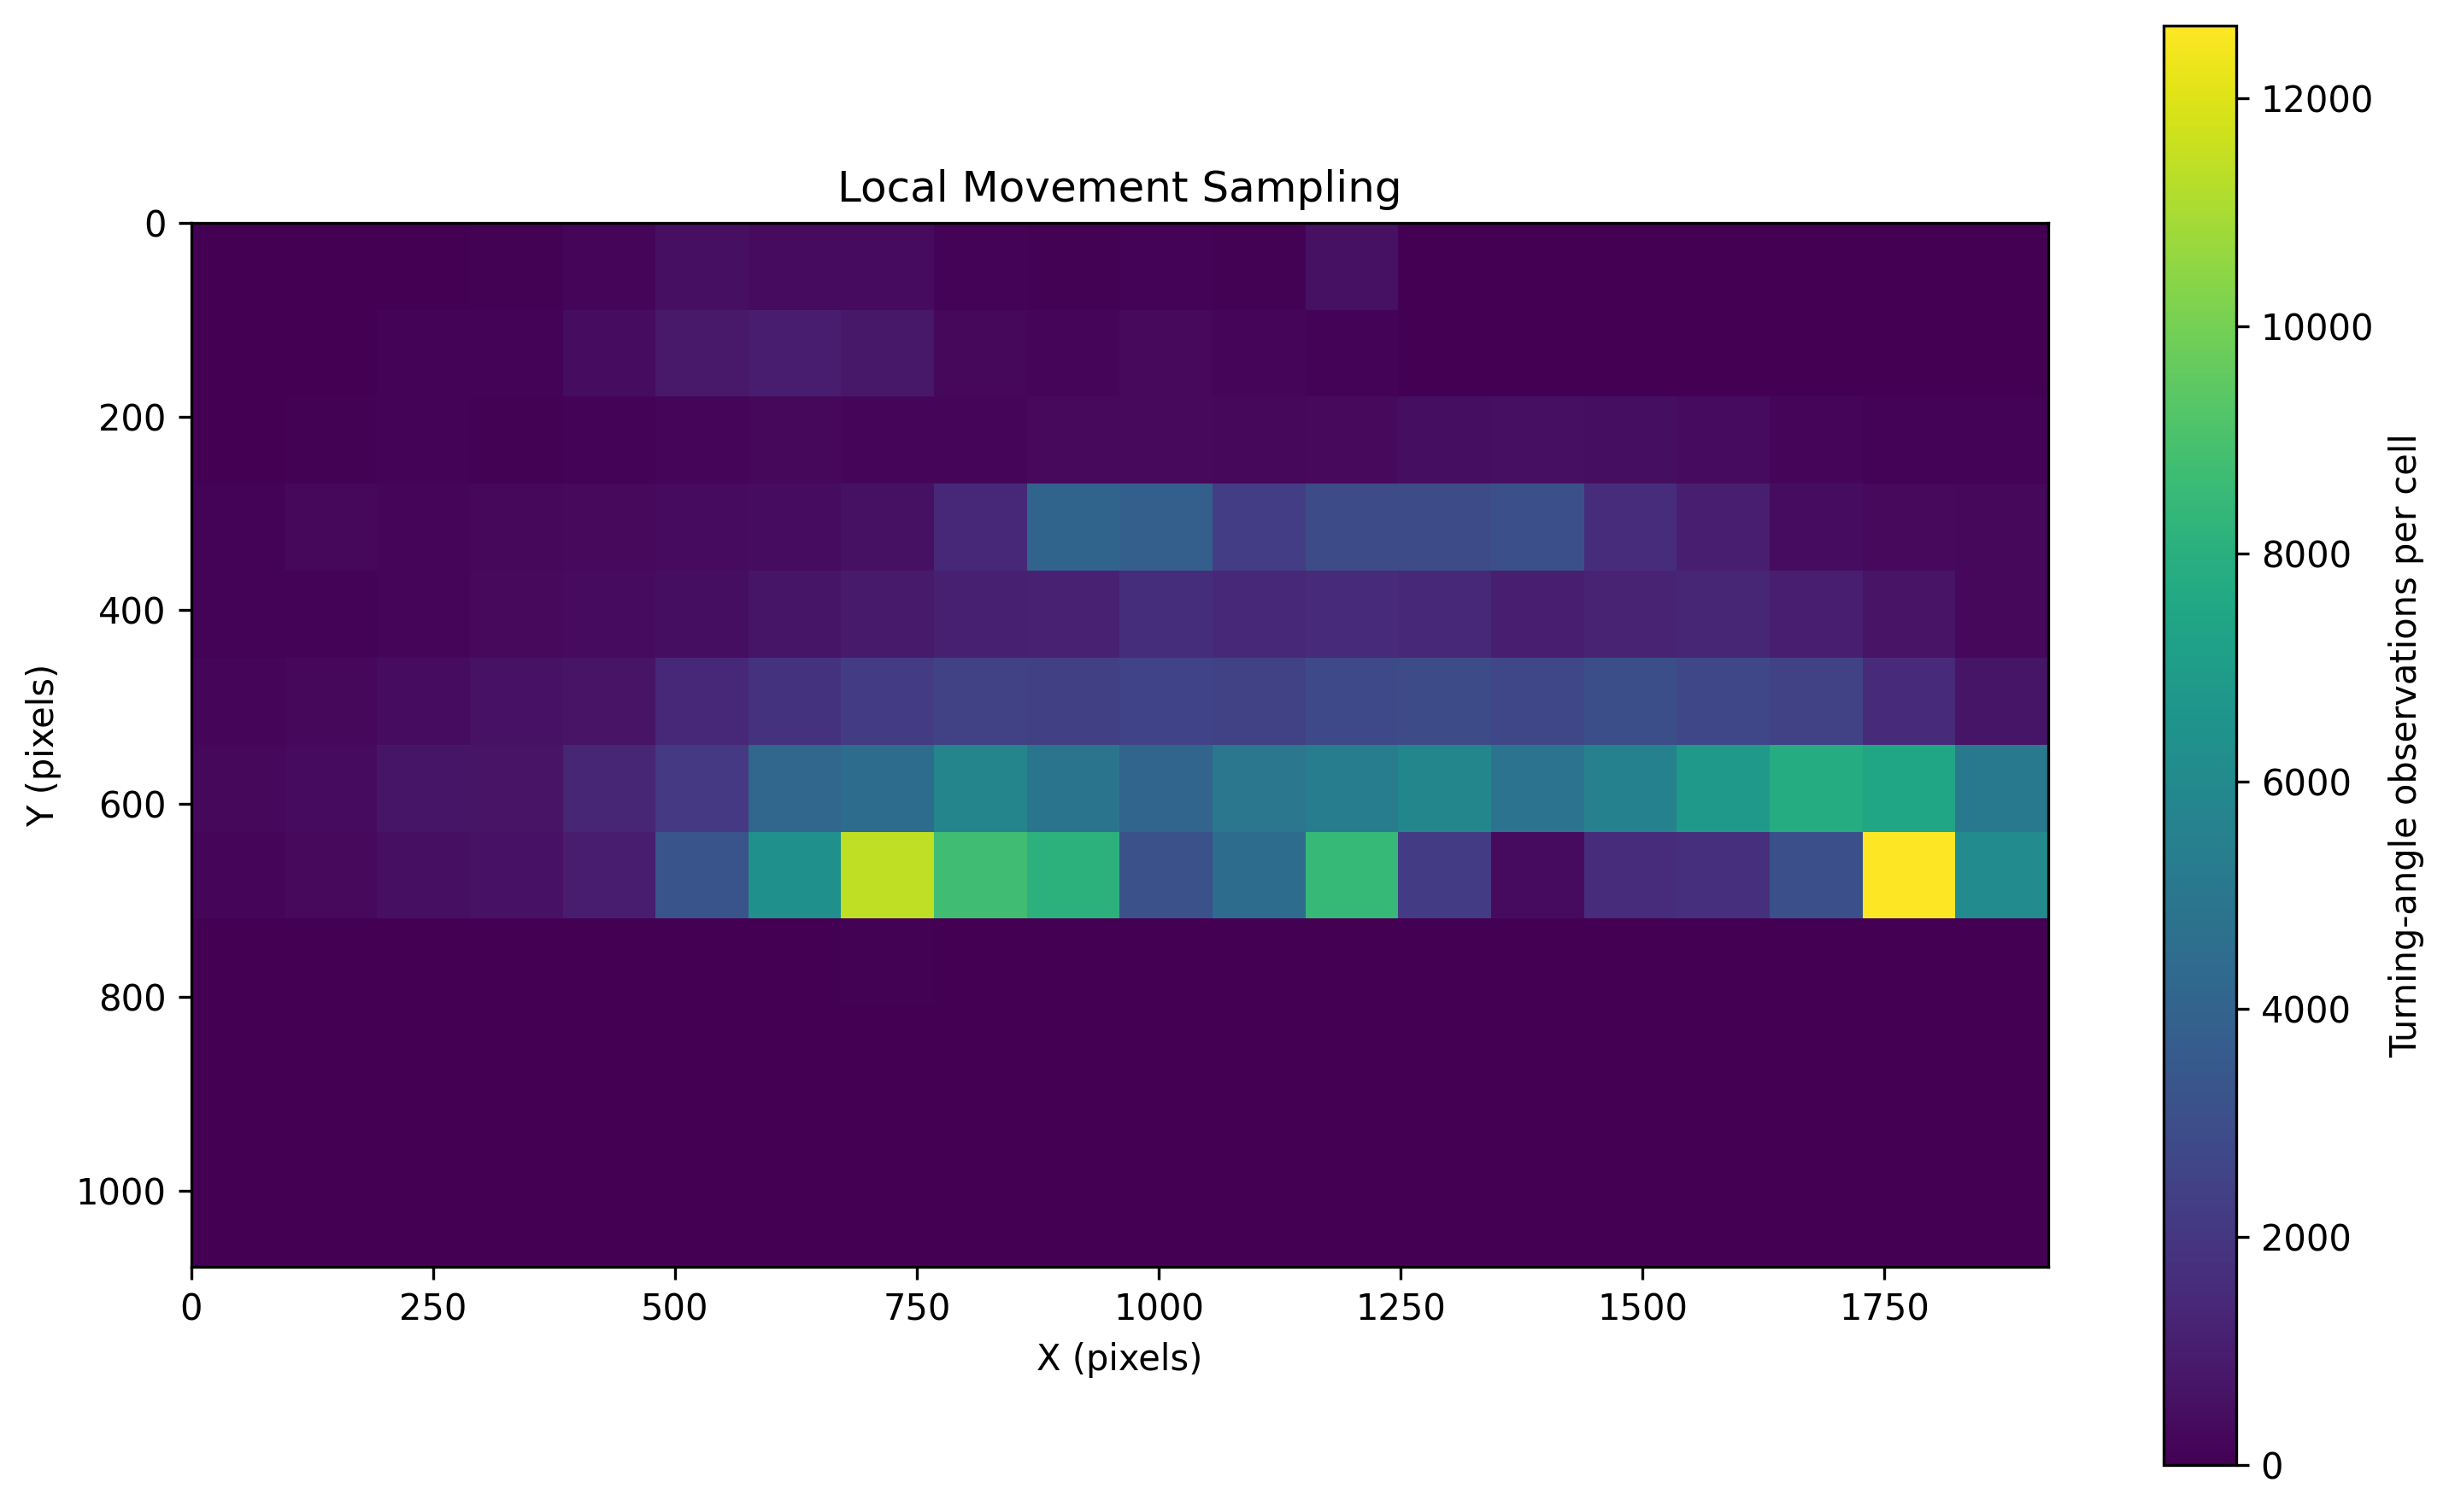
\includegraphics[width=0.78\textwidth]{figures/info_geometry_sampling_map.png}
\caption{Example spatial sampling map showing the number of valid turning-angle observations available in each grid cell. Cells below the configured minimum sample count are excluded from information-geometric comparisons.}
\label{fig:samplingmap}
\end{figure}

\subsection{Temporal Information Geometry}
With \texttt{--temporal-info-geometry}, the recording is divided into temporal windows. A turning-angle distribution is estimated for each sufficiently sampled window. BioTraj writes the complete temporal Fisher--Rao distance matrix and the distances between consecutive windows.

The window length controls temporal resolution. A sharp transition occurring inside a window produces a mixed distribution and may therefore yield the largest consecutive-window distance in the following comparison rather than exactly at the physical transition time.

\begin{figure}[H]
\centering
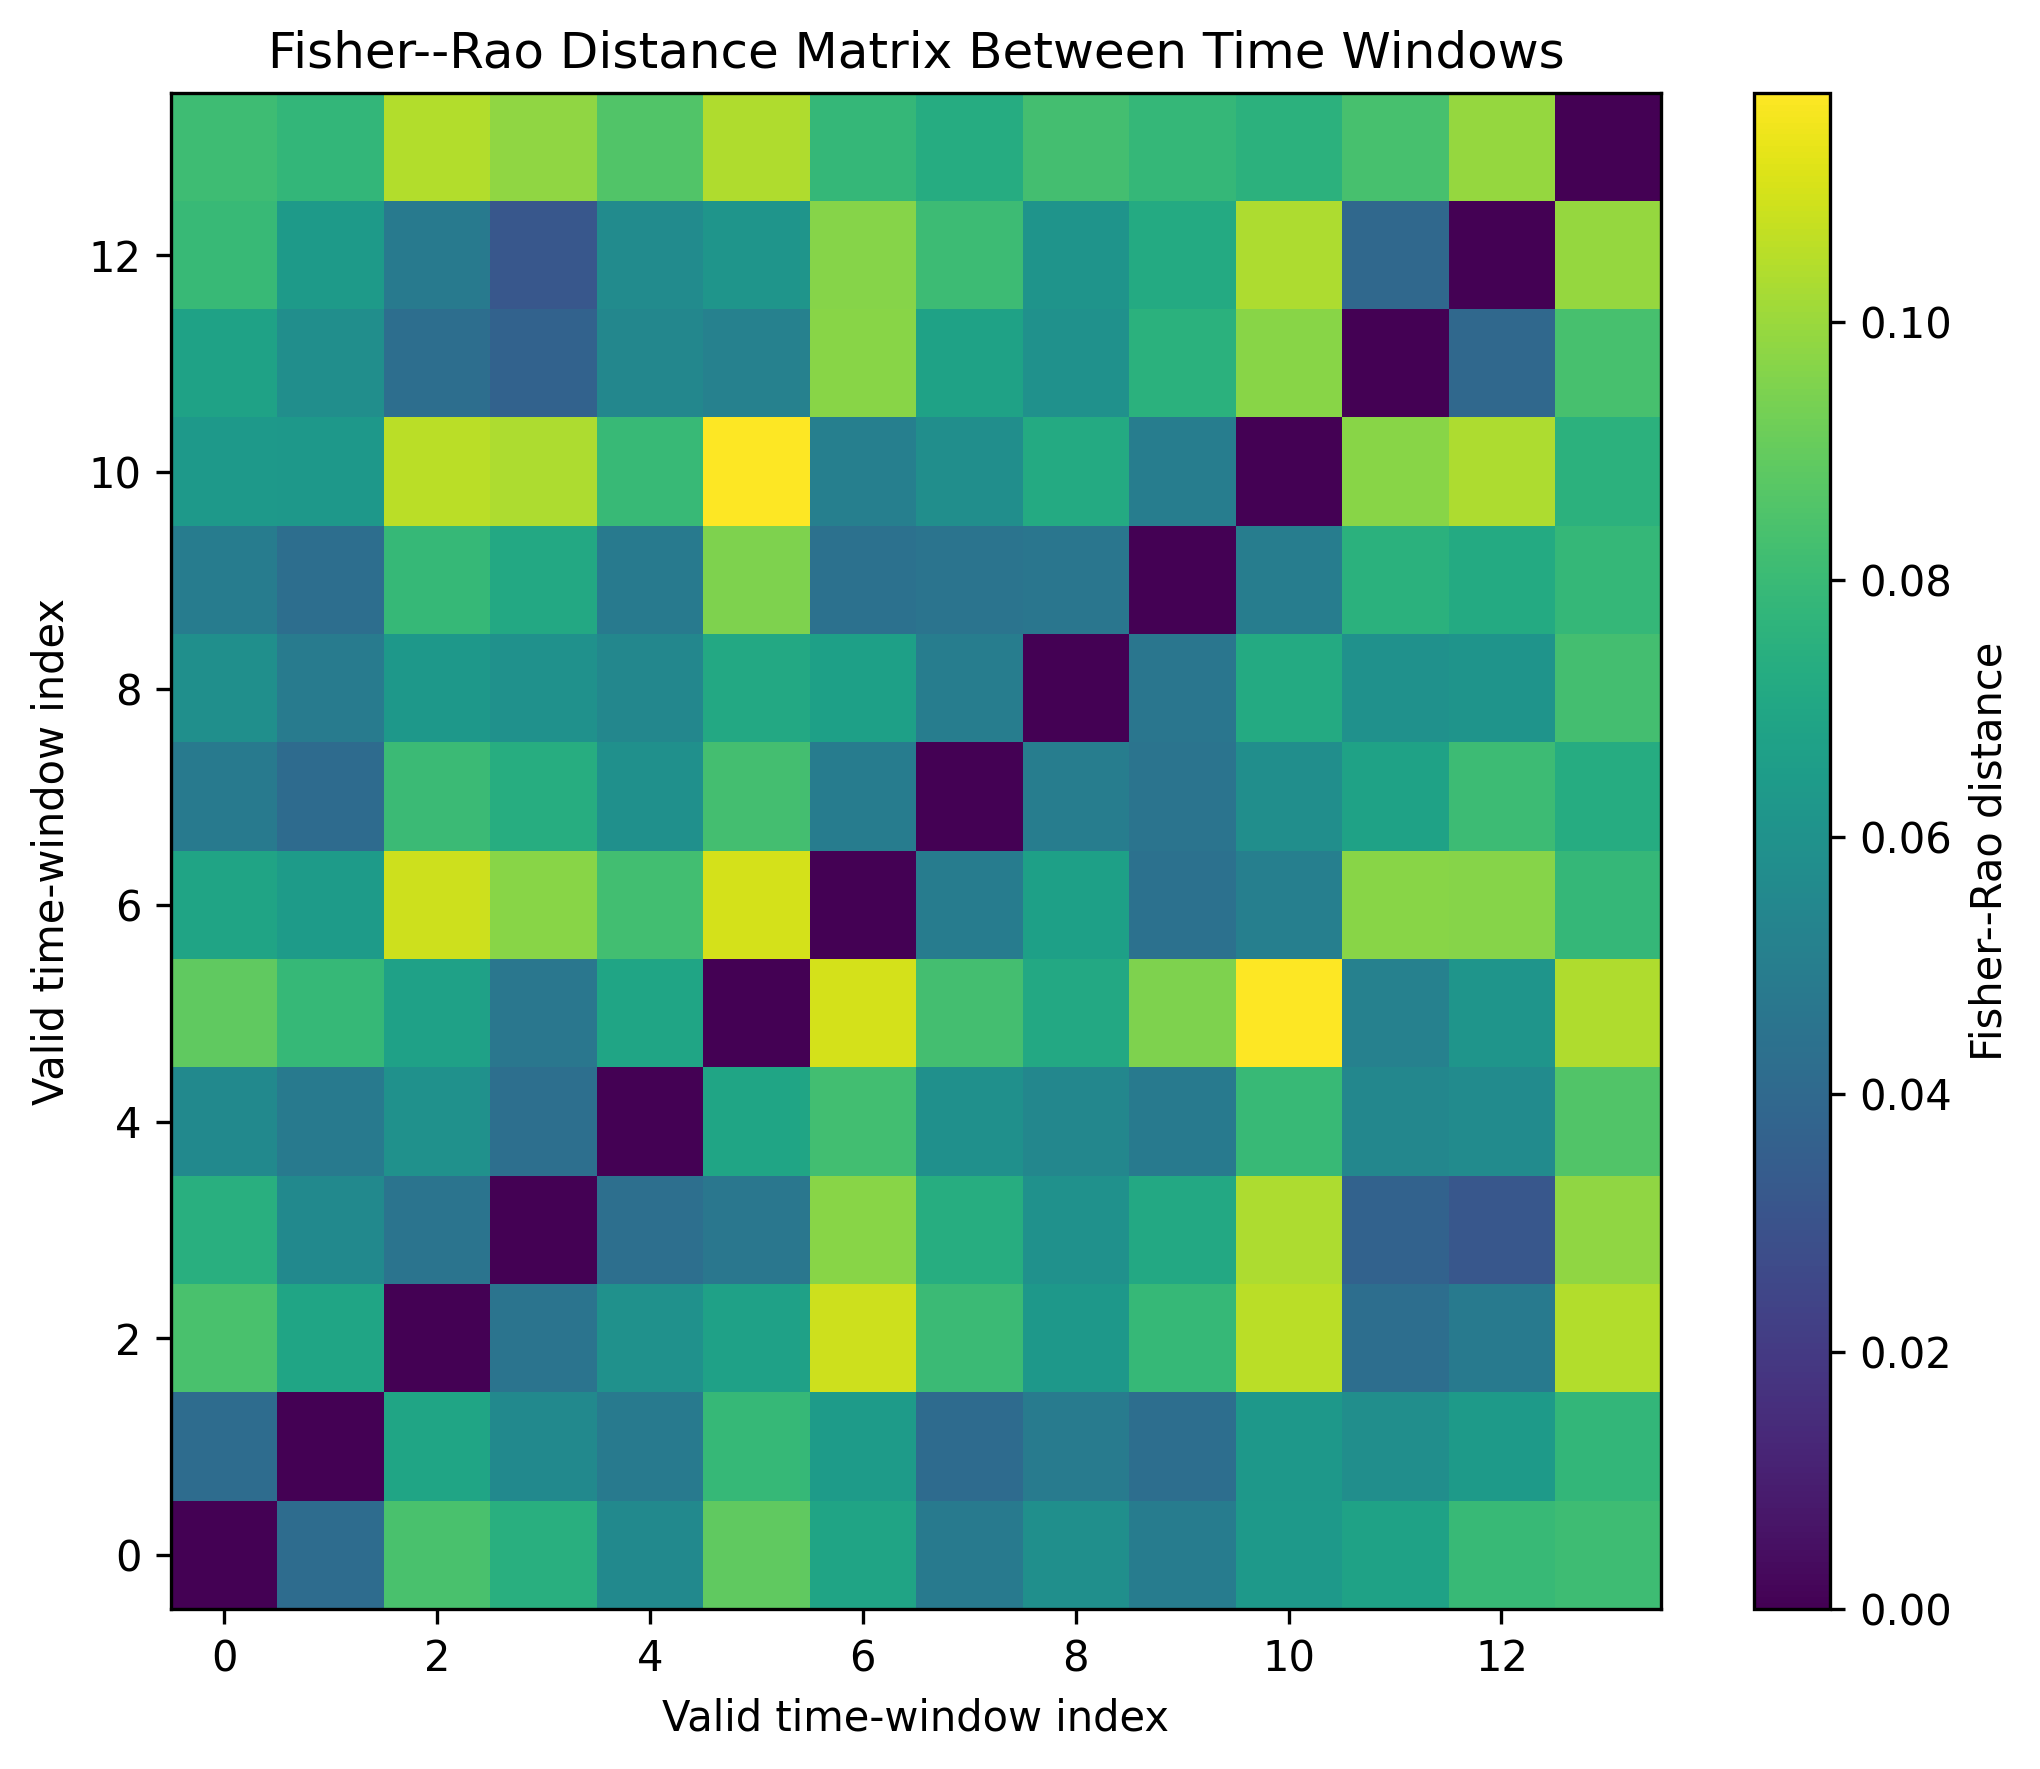
\includegraphics[width=0.72\textwidth]{figures/temporal_info_distance_matrix.png}
\caption{Example temporal Fisher--Rao distance matrix. Each element compares the turning-angle distributions estimated in two temporal windows.}
\label{fig:temporalmatrix}
\end{figure}

\begin{figure}[H]
\centering
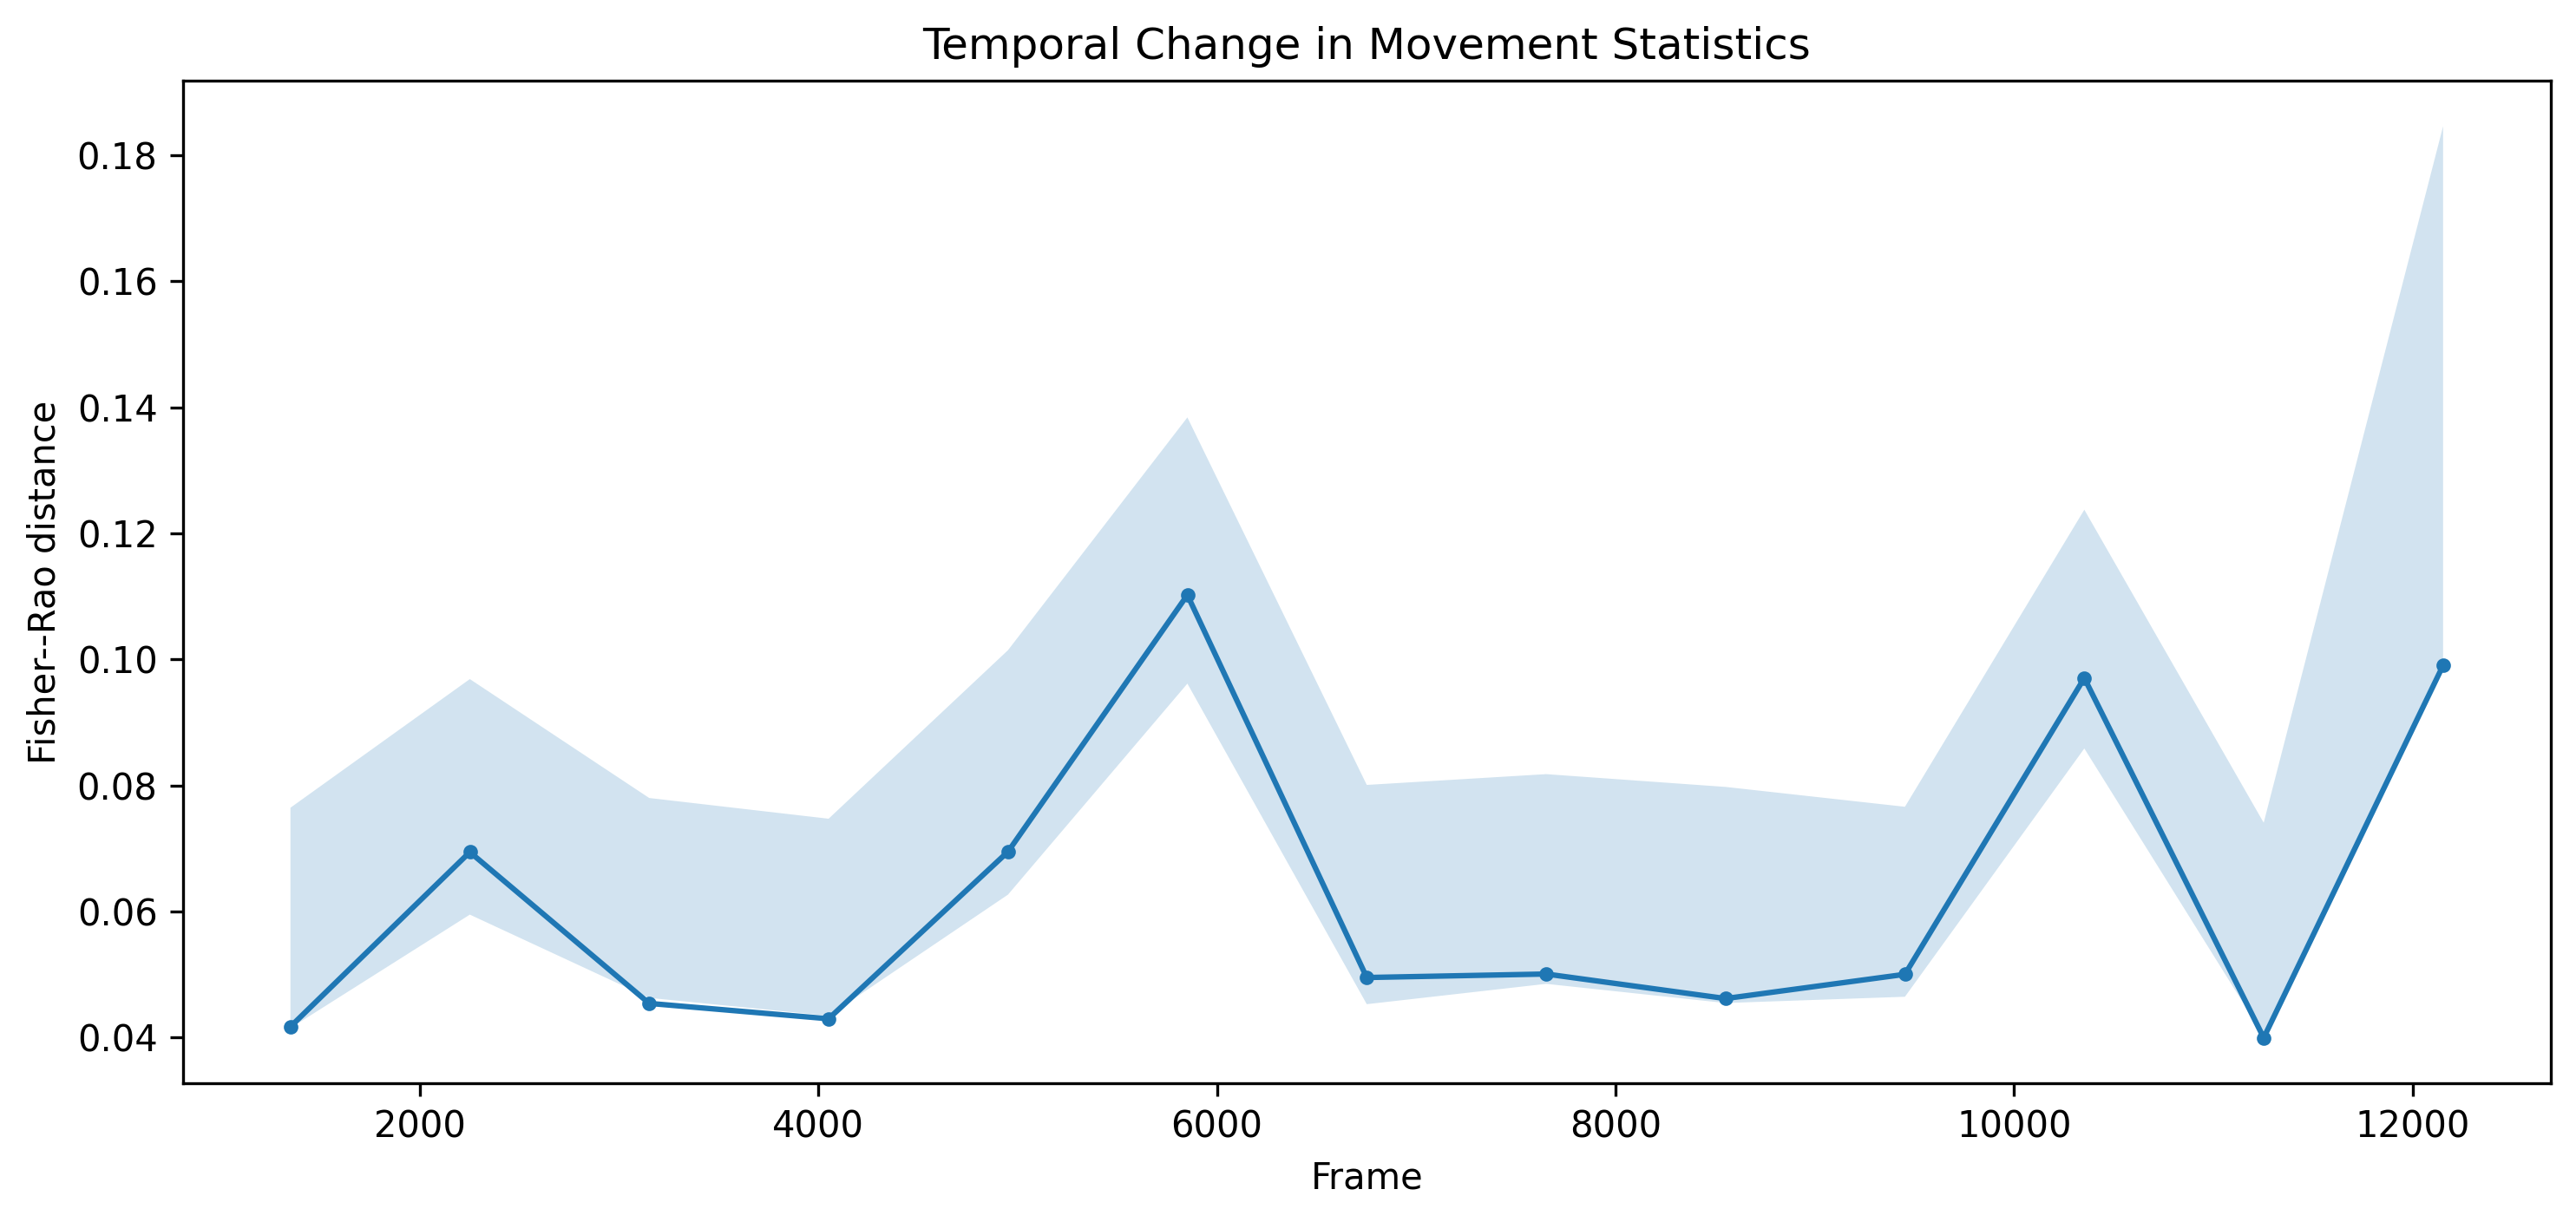
\includegraphics[width=0.78\textwidth]{figures/temporal_info_consecutive_distance.png}
\caption{Example consecutive-window Fisher--Rao analysis. Peaks identify periods in which the estimated movement distribution changes strongly between adjacent temporal windows.}
\label{fig:temporalconsecutive}
\end{figure}

\subsection{Bootstrap and Finite-Sampling Controls}

The spatial and temporal modules can bootstrap empirical turning-angle
samples to estimate uncertainty in Fisher--Rao distances. This quantifies
empirical sampling variability but does not make temporally correlated
observations or neighbouring spatial cells independent biological
replicates.

Raw Fisher--Rao values should not be compared across datasets with very
different local sample sizes without additional sampling controls.
BioTraj therefore supports interpretation using complementary diagnostics.
Equal-count resampling tests whether differences persist when the same
number of observations is used in each eligible spatial cell, whereas
threshold-convergence analysis examines the stability of the result as
the minimum number of observations required for a cell is increased.
Figure~\ref{fig:finitesampling} illustrates the equal-count approach.

\begin{figure}[H]
\centering
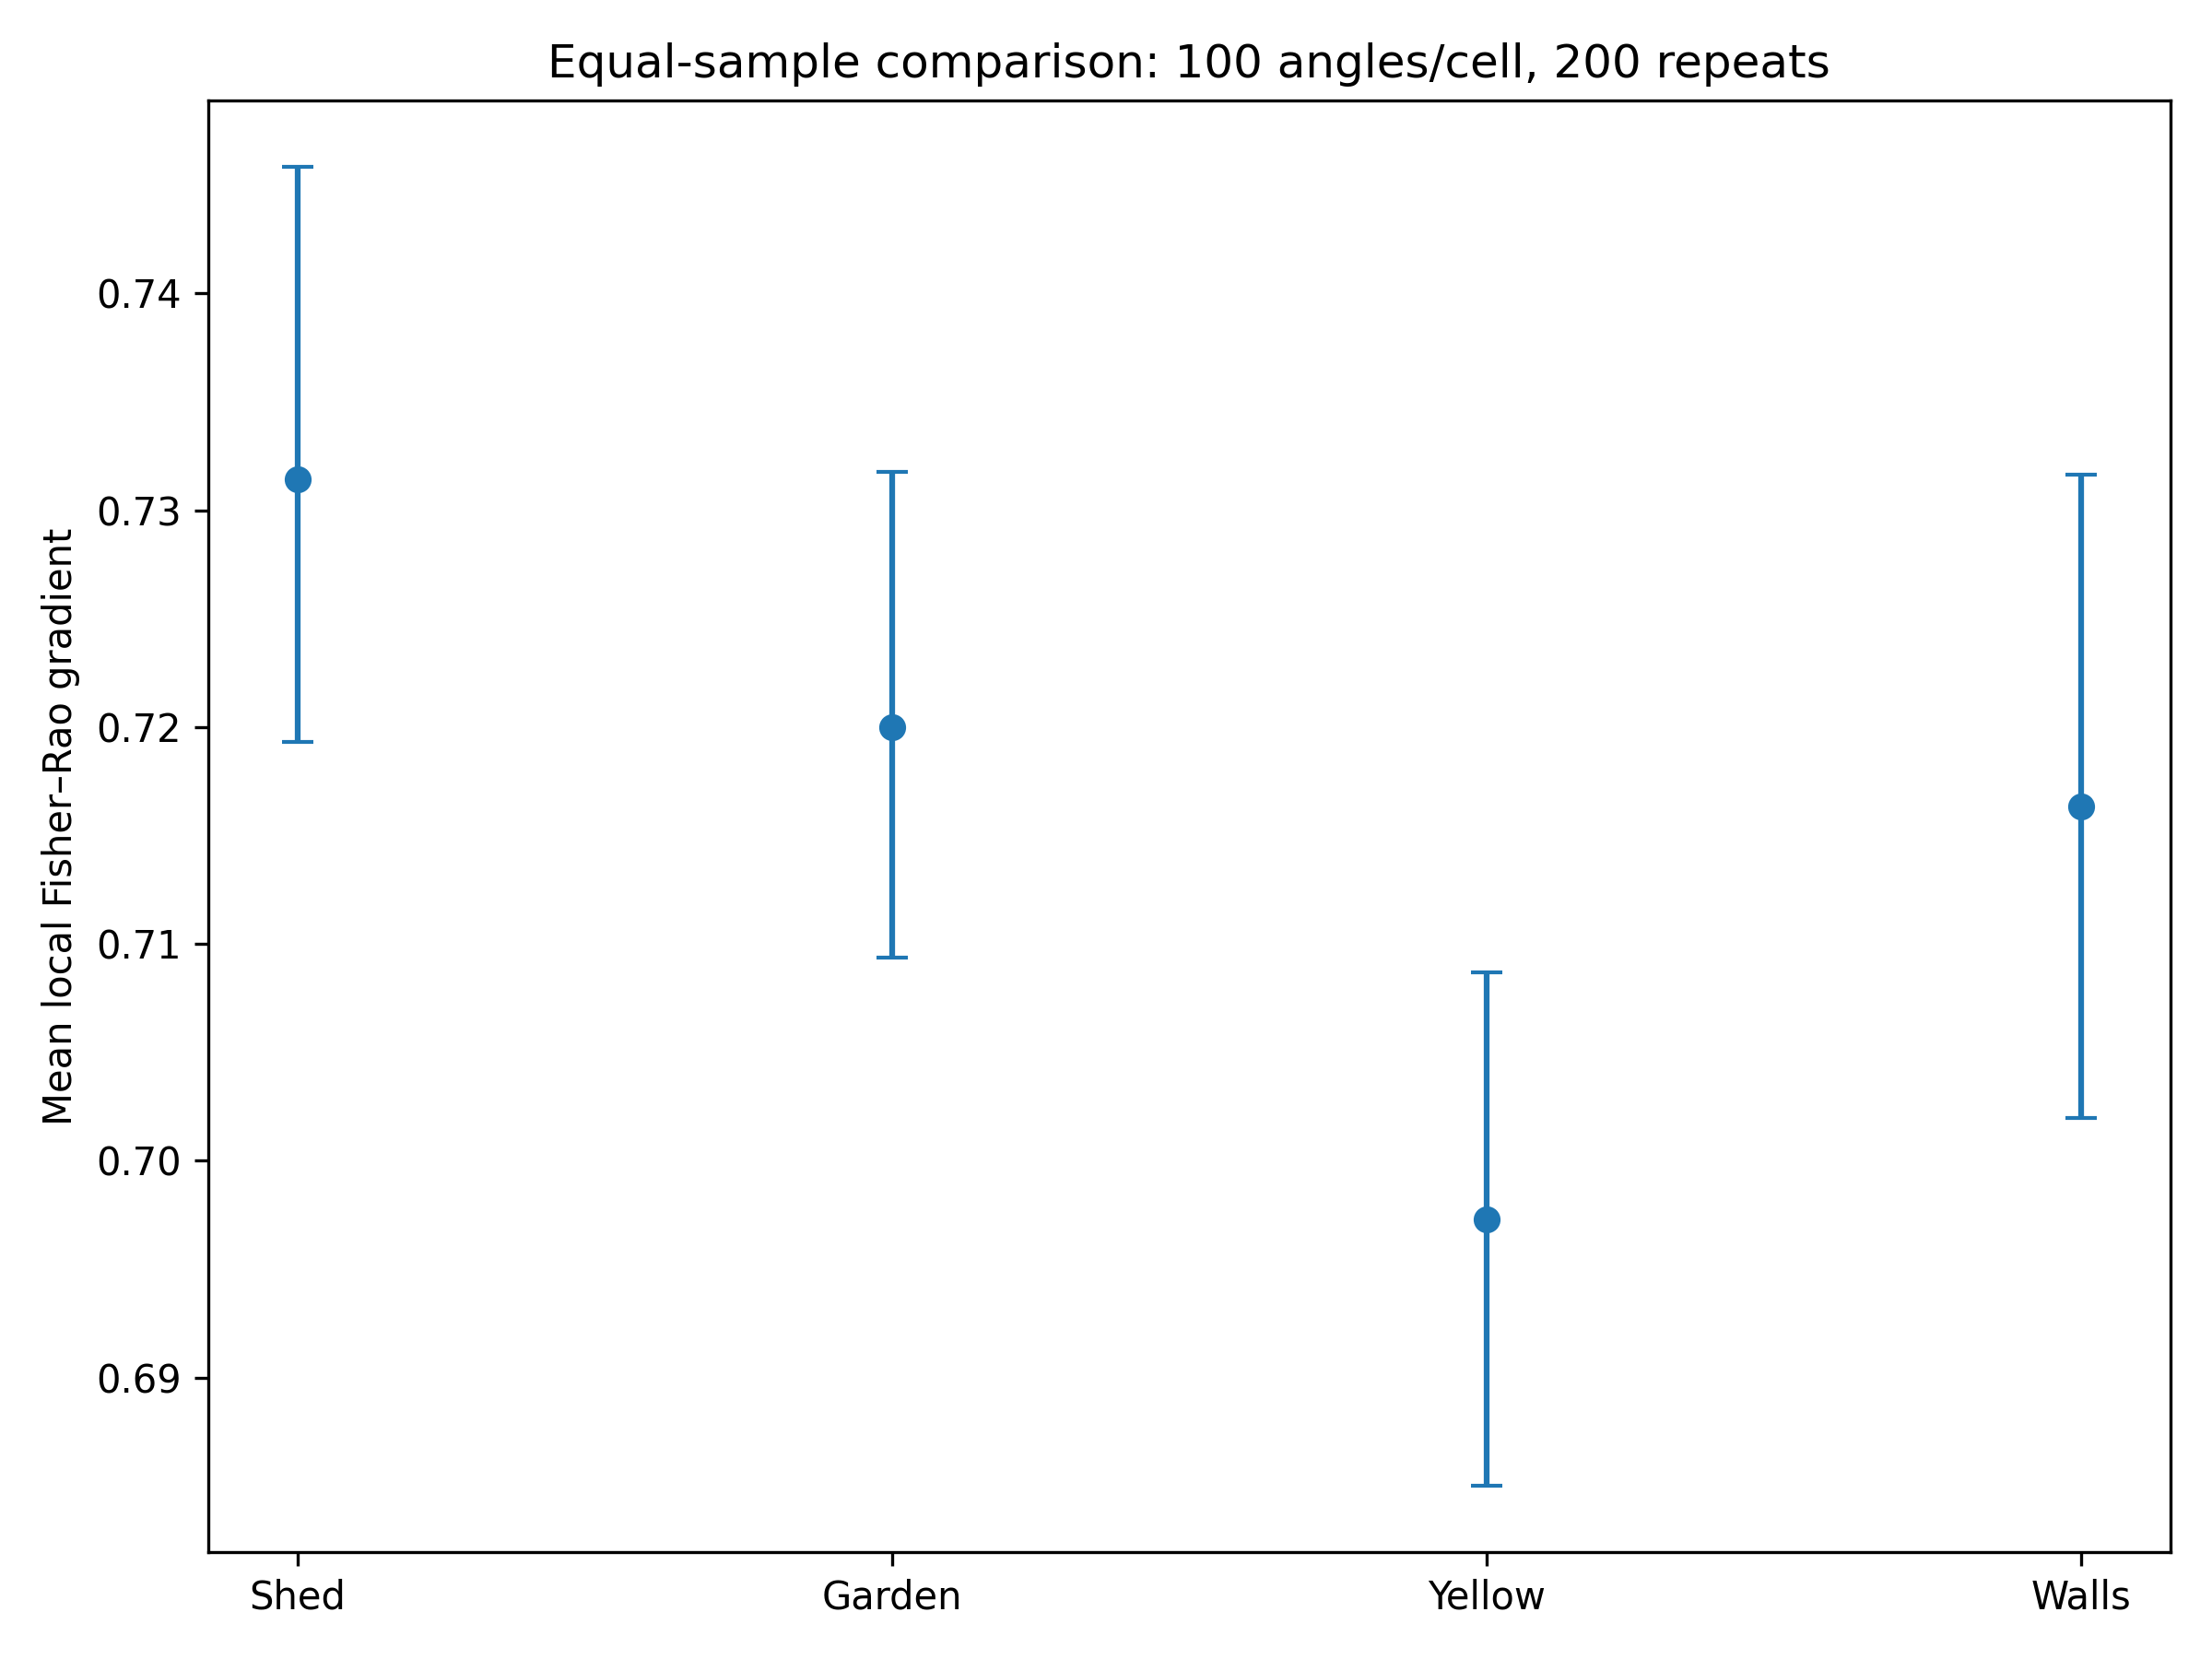
\includegraphics[width=0.82\textwidth] {figures/equal_sample_FR_comparison.png}
\caption{Equal-sample control for local Fisher--Rao heterogeneity.
Turning-angle observations are resampled to a common sample size before
calculating local Fisher--Rao quantities, reducing differences caused
solely by unequal numbers of observations among spatial cells. Repeated
resampling provides a measure of finite-sampling variability and helps
distinguish sampling effects from persistent differences among recordings.}
\label{fig:finitesampling}
\end{figure}

\section{Information-Geometry Command-Line Options}
The principal options in BioTraj v1.2 are summarized below.
\begin{longtable}{p{0.34\textwidth}p{0.15\textwidth}p{0.43\textwidth}}
\toprule
Option & Default & Meaning\\
\midrule
\endhead
\texttt{--info-geometry} & off & Enable spatial information geometry.\\
\texttt{--info-grid-x} & 20 & Number of spatial grid columns.\\
\texttt{--info-grid-y} & 12 & Number of spatial grid rows.\\
\texttt{--info-angle-bins} & 18 & Number of bins over $0$--$180^\circ$.\\
\texttt{--info-min-samples} & 30 & Minimum turning-angle observations per spatial cell.\\
\texttt{--info-clusters} & 4 & Number of hierarchical information-geometric distributional clusters. Clustering is optional/descriptive and does not define biological states.\\
\texttt{--info-pseudocount} & 0 & Optional pseudocount added per angular bin.\\
\texttt{--info-bootstrap} & 200 & Spatial bootstrap replicates; 0 disables bootstrap.\\
\texttt{--info-seed} & 12345 & Random seed for information-geometry bootstrap.\\
\texttt{--temporal-info-geometry} & off & Enable temporal information geometry.\\
\texttt{--temporal-window-frames} & 1800 & Temporal window length in frames.\\
\texttt{--temporal-step-frames} & window length & Step between temporal windows.\\
\texttt{--temporal-min-samples} & 100 & Minimum turning-angle observations per temporal window.\\
\texttt{--temporal-bootstrap} & 200 & Temporal bootstrap replicates; 0 disables bootstrap.\\
\texttt{--fps} & none & Frame rate; when supplied, temporal axes can be expressed in seconds.\\
\bottomrule
\end{longtable}

\section{Reproducing the Information-Geometry Settings Used in the BioTraj Study}
The analyses reported with BioTraj v1.2 used a $20\times12$ spatial grid, 18 turning-angle bins, a minimum of 30 angles per spatial cell, 200 bootstrap replicates, and 15-s non-overlapping temporal windows for 60-fps recordings. Because the program default temporal window is 1800 frames, the 900-frame manuscript setting must be supplied explicitly:
\begin{lstlisting}
python3 AntTrajectoryAnalysis.py \
    ant_tracks.csv \
    --output BioTraj_V1_2_results \
    --info-geometry \
    --info-grid-x 20 \
    --info-grid-y 12 \
    --info-angle-bins 18 \
    --info-min-samples 30 \
    --info-clusters 4 \
    --info-pseudocount 0 \
    --info-bootstrap 200 \
    --info-seed 12345 \
    --temporal-info-geometry \
    --temporal-window-frames 900 \
    --temporal-step-frames 900 \
    --temporal-min-samples 100 \
    --temporal-bootstrap 200 \
    --fps 60
\end{lstlisting}

\subsection{Synthetic Validation Data}

BioTraj v1.2 includes the controlled trajectory generator
\texttt{BioTraj\_SyntheticTrajectoryGenerator\_v1\_2\_structured\_arena.py}.
The generator produces synthetic trajectories for which the underlying
spatial and/or temporal statistical structure is known in advance. These
datasets provide a controlled test of the information-geometric analysis
independently of experimental tracking uncertainty.

The generator contains five scenarios:
\begin{enumerate}
\item \textbf{Homogeneous stationary}: the same movement law is used
throughout the arena and throughout the recording;
\item \textbf{Spatial two-domain}: the movement law changes across a known
vertical spatial boundary;
\item \textbf{Temporal two-state}: the movement law changes at a known frame;
\item \textbf{Spatiotemporal}: spatial domains are combined with a known
temporal change;
\item \textbf{Structured arena}: a localization benchmark containing a
circular nest/entrance zone, a directional corridor, a wall/surface-transition
boundary, and ordinary observation-frame exits.
\end{enumerate}

The first four scenarios correspond to the controlled synthetic validation
cases used in the BioTraj study. The structured-arena case is an additional
validation example distributed with BioTraj v1.2. Its semantic geometry is
stored as ground truth but is not supplied to the BioTraj information-geometric
analysis.

The synthetic movement model updates the direction according to a von Mises
turning distribution and draws positive step lengths from a truncated normal
distribution. It is intentionally a controlled validation model rather than a
realistic mechanistic model of ant behaviour.

To generate all supplied validation scenarios without automatically launching
the BioTraj analysis, use for example:
\begin{lstlisting}
python3 BioTraj_SyntheticTrajectoryGenerator_v1_2.py \
    --all \
    --base-dir synthetic_validation \
    --seed 12345 \
    --generate-only
\end{lstlisting}

Each generated scenario contains an \texttt{ant\_tracks.csv} file compatible
with \texttt{AntTrajectoryAnalysis.py}, together with configuration and
ground-truth metadata and a trajectory preview. The generated trajectories can
therefore be passed through the same analysis workflow used for experimental
data.

For the validation cases reported in the BioTraj study, the synthetic
trajectories used 20 agents, 12,116 frames, a $1905\times726$ pixel arena,
60 frames s$^{-1}$, and random seed 12345. The imposed spatial and temporal
changes are known independently of the information-geometric analysis, allowing
recovery of these changes to be assessed at the resolution of the selected
spatial grid and temporal windows.

\begin{figure}[H]
\centering

\begin{minipage}{0.48\textwidth}
    \centering
    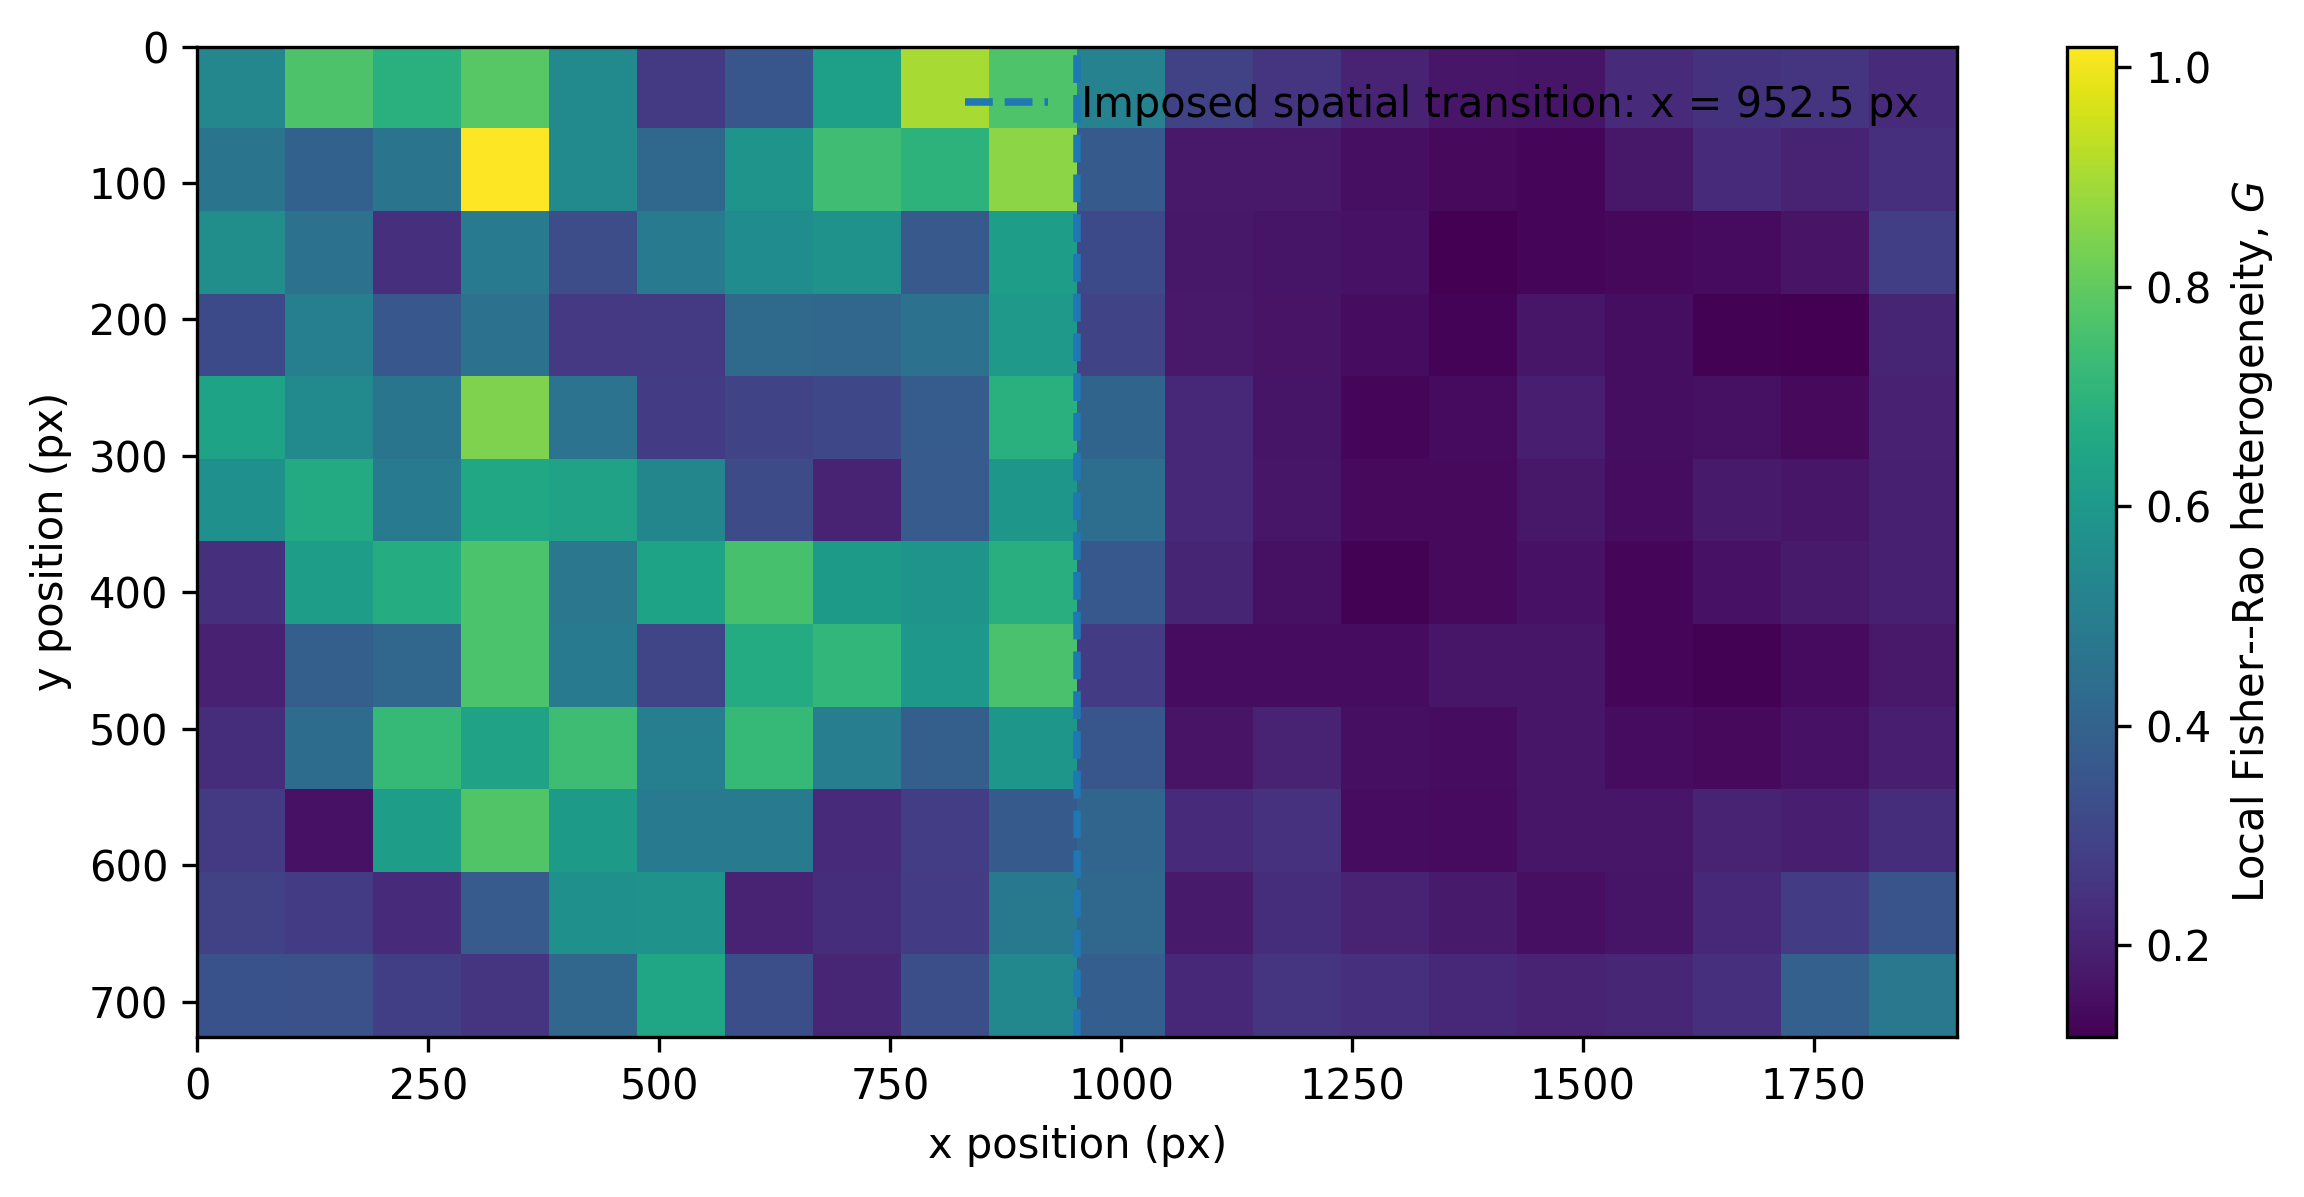
\includegraphics[width=\textwidth]
    {figures/SI_S5a_spatial_FR_validation.png}

    \textbf{(a) Spatial validation}
\end{minipage}
\hfill
\begin{minipage}{0.48\textwidth}
    \centering
    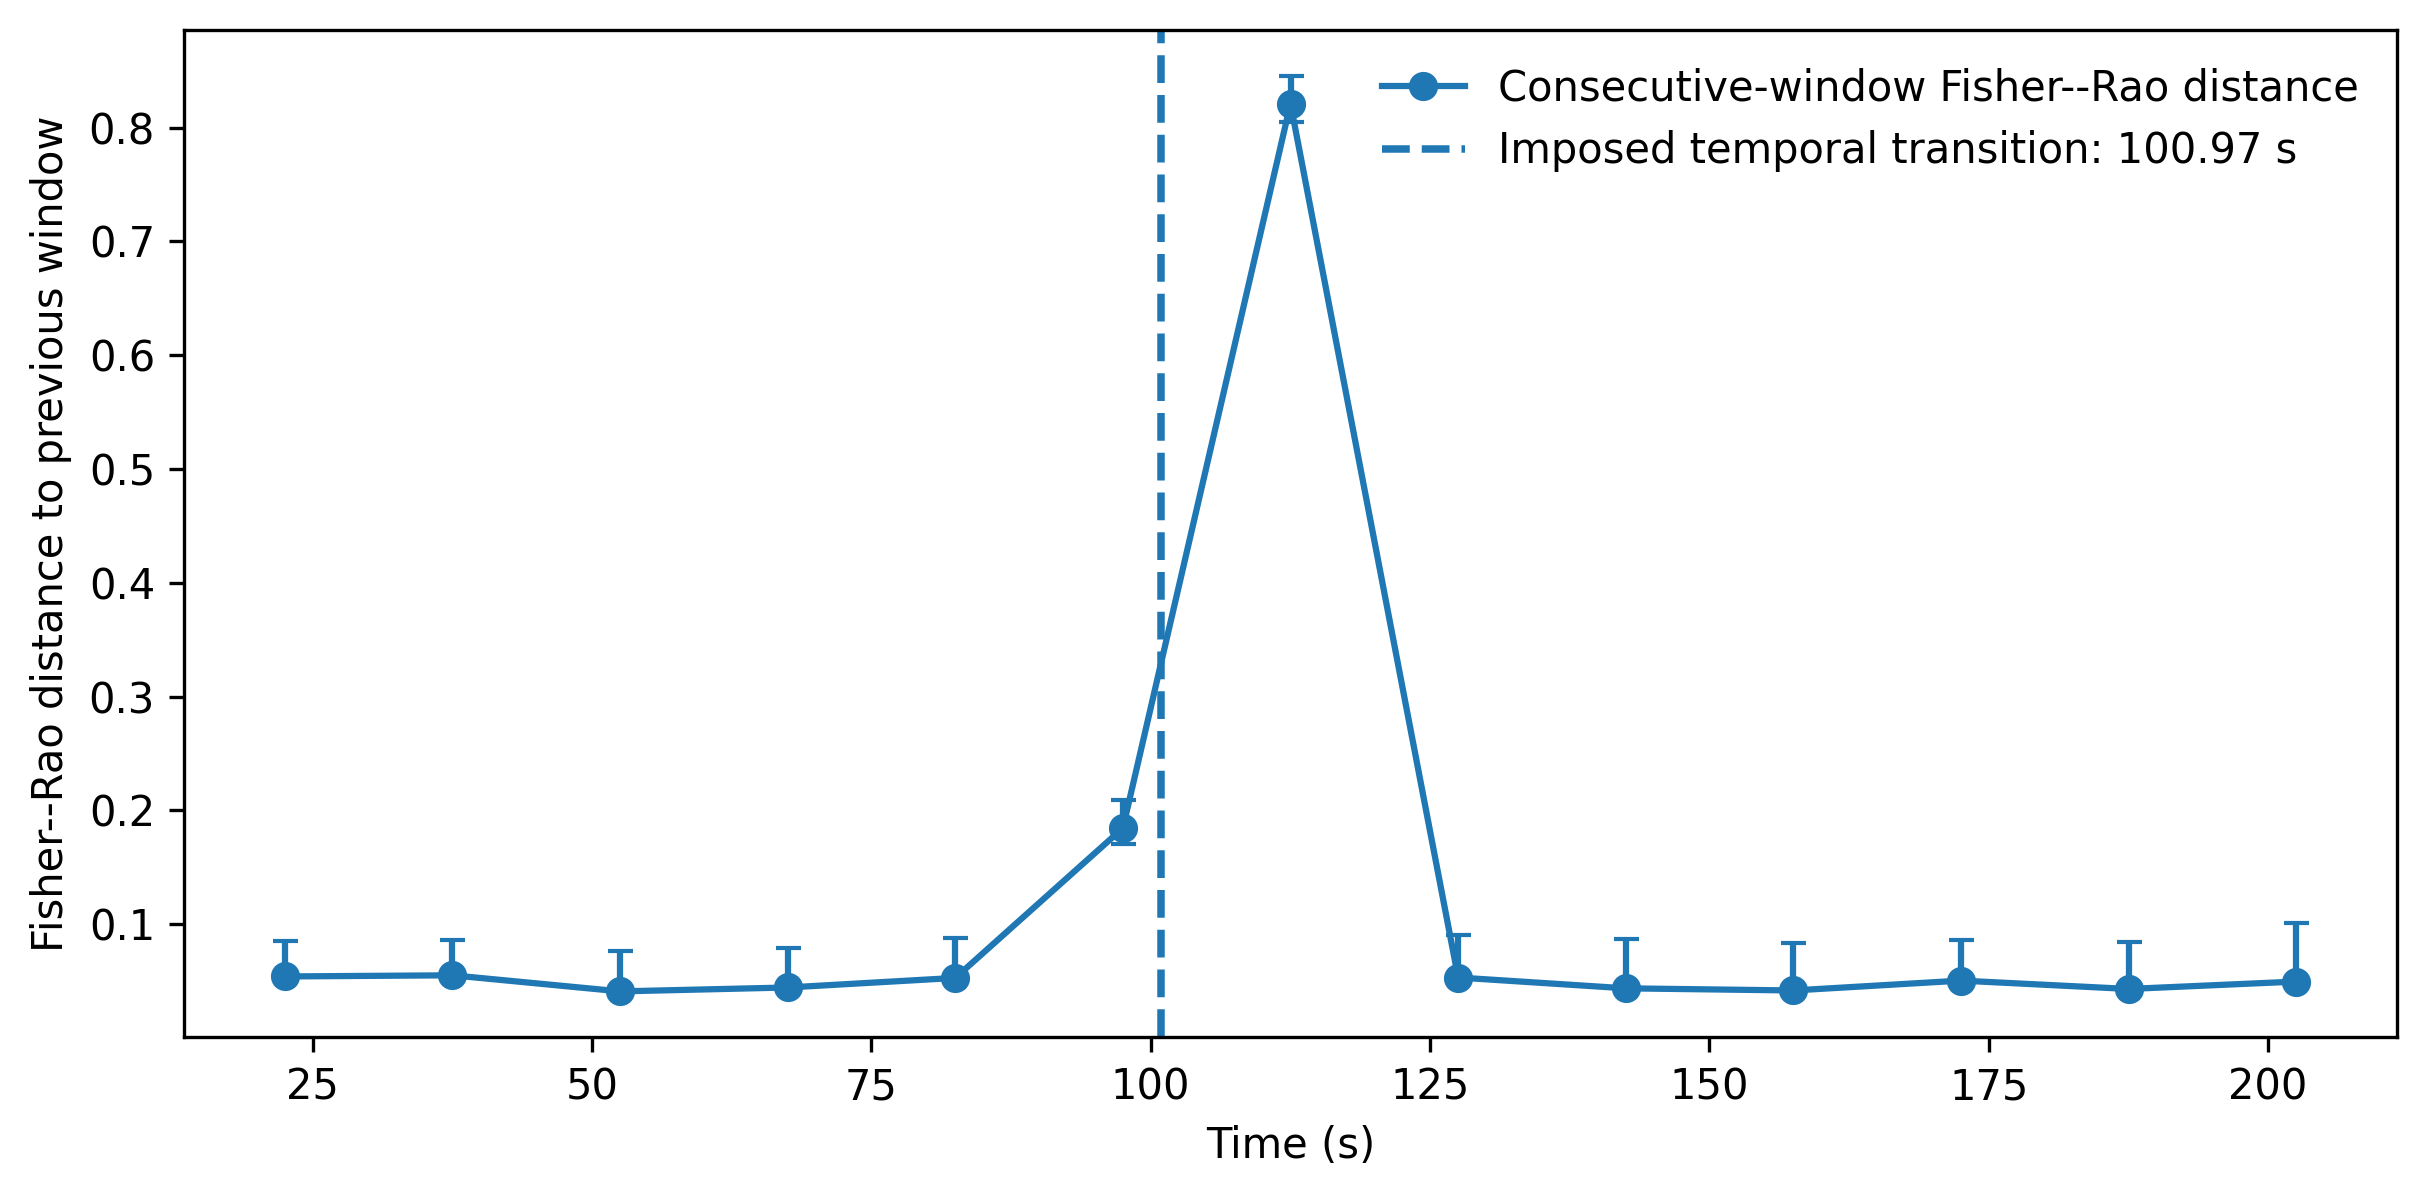
\includegraphics[width=\textwidth]
    {figures/SI_S5b_temporal_FR_validation.png}

    \textbf{(b) Temporal validation}
\end{minipage}

\caption{\textbf{Simulation-based validation of the information-geometric
analysis.}
(a) Spatial validation using synthetic trajectories with a known change
in movement statistics across the arena. The spatial Fisher--Rao analysis
is evaluated against the imposed spatial structure.
(b) Temporal validation using synthetic trajectories with a known change
in movement statistics during the recording. The temporal Fisher--Rao
analysis is evaluated against the imposed transition time.
Because the spatial and temporal changes are specified independently when
the trajectories are generated, these tests provide controlled validation
of the ability of BioTraj to recover distributional heterogeneity at the
resolution of the selected spatial grid and temporal windows.}

\label{fig:simulation}
\end{figure}

\section{Information-Geometry Output Files}
Depending on enabled options, the v1.2 analysis writes numerical tables, summaries, and figures. Important information-geometric outputs include:
\begin{itemize}
\item \texttt{info\_geometry\_cells.csv}: cell-level spatial information-geometry results;
\item \texttt{info\_geometry\_summary.json}: spatial analysis settings and summary quantities;
\item spatial sampling, local Fisher--Rao gradient, distance-matrix, and distributional-cluster figures;
\item \texttt{temporal\_info\_windows.csv}: window-level temporal information;
\item \texttt{temporal\_fisher\_rao\_distance\_matrix.csv}: complete temporal distance matrix;
\item \texttt{temporal\_info\_geometry\_summary.json}: temporal settings and summary information;
\item temporal sampling, distance-matrix, and consecutive-distance figures.
\end{itemize}
File names can evolve slightly between development builds; the release version and its generated summary files should be retained with published analyses.

\section{Scene Annotation and Annotation-Aware Analysis}

The supplied \texttt{examples/WallAnts/} dataset illustrates the complete
three-stage workflow. Tracking outputs are stored in
\texttt{tracking\_results/}, conventional and information-geometric analysis
outputs in \texttt{BioTraj\_V1\_2\_revision2/}, and the annotation-aware
Fisher--Rao results in \texttt{WALL\_annotated\_FR\_v1\_1/}. The example also
includes \texttt{FirstFrame.jpg}, the corresponding scene-annotation JSON
file, and an annotated reference image.



BioTraj v1.2 includes two companion utilities for relating independently
defined features of the recorded scene to the spatial Fisher--Rao results:
\texttt{BioTraj\_Scene\_Annotator.py} and
\texttt{BioTraj\_Annotated\_FR\_Analysis\_v1\_1.py}. These utilities are
separate from the main trajectory-analysis program so that physical or
biological scene information can be defined independently of the
information-geometric result.

\subsection{Scene Annotation}

The graphical scene annotator can be started with:
\begin{lstlisting}
python3 BioTraj_Scene_Annotator.py FirstFrame.jpg
\end{lstlisting}
where \texttt{FirstFrame.jpg} is a reference image in the same coordinate
system as the tracked trajectories.

The annotator stores scene information in JSON format using original-image
pixel coordinates. It can be used to define polygonal regions, polylines,
circles, surface regions, surface transitions, biological features, physical
constraints, observation boundaries, and artifact or exclusion regions.

Three concepts should remain distinct:
\begin{center}
\textbf{tracking domain} $\neq$
\textbf{biological/physical regions} $\neq$
\textbf{artifact masks}.
\end{center}

Whenever possible, scene annotations intended for biological or physical
interpretation should be defined independently of the Fisher--Rao map. This
reduces the risk of selecting regions retrospectively because they coincide
with features already visible in the information-geometric result.

\subsection{Annotation-Aware Fisher--Rao Analysis}

The annotation-aware analysis combines the scene-annotation JSON file with
\texttt{info\_geometry\_cells.csv} generated by
\texttt{AntTrajectoryAnalysis.py}. A typical command is:
\begin{lstlisting}
python3 BioTraj_Annotated_FR_Analysis_v1_1.py \
    --annotations FirstFrame_scene_annotations.json \
    --info-cells BioTraj_results/info_geometry_cells.csv \
    --tracks ant_tracks.csv \
    --image FirstFrame.jpg \
    --grid-x 20 \
    --grid-y 12 \
    --output annotated_FR_results
\end{lstlisting}

The \texttt{--tracks} argument is optional but is recommended when the
original BioTraj image frame should be inferred consistently. The
\texttt{--image} argument is optional and supplies a reference image for
registration and Fisher--Rao overlays. The explicit \texttt{--grid-x} and
\texttt{--grid-y} values are strongly recommended when
\texttt{info\_geometry\_cells.csv} contains only the populated/valid cells,
because they preserve the full spatial grid used by the original analysis.

The program assigns valid information-geometric cells to annotated scene
features and produces regional and transition-based summaries. It can also
evaluate local Fisher--Rao heterogeneity as a function of distance from
annotated transitions and generate graphical overlays and quality-control
outputs. Regions marked for exclusion in the annotation file can be treated
as artifact masks in the corresponding quality-controlled summaries.

Annotation-aware comparisons remain descriptive unless the experimental
design provides genuine independent biological replication. Spatial cells
within one recording should not automatically be treated as independent
biological replicates, and a relationship between Fisher--Rao heterogeneity
and an annotated feature does not by itself establish a biological mechanism.

\subsection{Annotation-Aware Workflow}

The intended sequence is:
\begin{enumerate}
\item extract trajectories with \texttt{AntTracking.py}, or provide compatible
trajectory data from another tracker;
\item analyse the trajectories with \texttt{AntTrajectoryAnalysis.py} and
generate \texttt{info\_geometry\_cells.csv};
\item select a reference image, normally the first video frame;
\item define scene features independently using
\texttt{BioTraj\_Scene\_Annotator.py};
\item combine the annotation JSON file and the spatial information-geometric
results using \texttt{BioTraj\_Annotated\_FR\_Analysis\_v1\_1.py};
\item inspect both raw and quality-controlled regional/transition summaries
before biological interpretation.
\end{enumerate}

\section{Recommended Analysis Workflow}
A robust information-geometric workflow is:
\begin{enumerate}
\item inspect tracking quality and preserve continuous track segments;
\item inspect occupancy and conventional trajectory descriptors;
\item inspect the spatial sampling map;
\item calculate spatial and/or temporal Fisher--Rao results using justified minimum sample counts;
\item inspect bootstrap uncertainty and finite-sampling diagnostics;
\item relate detected statistical structure to independently defined scene information where appropriate;
\item avoid assigning biological mechanisms or behavioural states from Fisher--Rao values alone.
\end{enumerate}

\section{Limitations}
The current implementation primarily assumes two-dimensional motion in the imaging plane. Tracking can be affected by poor contrast, object overlap, illumination changes, out-of-plane motion, and projection effects. Information-geometric estimates additionally depend on histogram resolution, spatial/temporal partitioning, and finite sample size. Spatial cells and temporal observations from a single recording are generally correlated and should not automatically be treated as independent biological replicates.

\section{Applications}
BioTraj can be adapted to ants and other social insects, protozoa, rotifers, nematodes, slugs and snails, small aquatic organisms, active-matter experiments, and simulated or robotic agents. Suitability depends on whether reliable trajectories can be reconstructed at a spatial and temporal resolution appropriate to the biological question.

\section{Citation and Reproducibility}
If BioTraj is used in academic work, cite the associated publication and the archived/released version of the BioTrajectoryAnalysis repository. For reproducibility, record the software release or commit, command-line options, random seed, input trajectory file, frame rate, calibration, and any scene-annotation files used in interpretation.

\section{License}
BioTraj is distributed under the MIT License.

\end{document}
